\noindent Im zeitkontinuierlichen Bereich werden dynamische Systeme mit Differentialgleichungen beschrieben. F\"{u}r zeitdiskrete Systeme geht die Differentiation in einen Differenzenquotienten \"{u}ber. Daraus resultiert die Beschreibung zeitdiskreter Systeme mit Differenzengleichungen. \medskip

\noindent Zu Beginn des Kapitels werden einige typische zeitdiskrete Systeme beschrieben und die Systemantworten mit numerischen Algorithmen bestimmt. Als Beispiele werden ein rekursives Filter, ein System mit einer gleitenden Mittelwertrechnung und eine Switched-Capacitor-Schaltung diskutiert. F\"{u}r die Systeme werden die jeweiligen Differenzengleichungen aufgestellt, diskutiert und numerisch gel\"{o}st.\medskip

\noindent Lineare, zeitinvariante Systeme haben im zeitkontinuierlichen Bereich eine besonders anschauliche L\"{o}sung und Interpretation erm\"{o}glicht. Der Begriff des linearen, zeitinvarianten Systems existiert auch f\"{u}r zeitdiskrete Systeme. Im zweiten Abschnitt dieses Kapitels werden grundlegende Systemeigenschaften erl\"{a}utert und Verfahren zum Nachweis der unterschiedlichen Eigenschaften vorgestellt.\medskip

\noindent Numerische L\"{o}sungen von Differenzengleichungen eignen sich nicht f\"{u}r eine analytische Bestimmung von Systemeigenschaften. Deshalb ist es erforderlich, analytische L\"{o}sungsmethoden zu diskutieren. Im dritten Abschnitt wird die analytische Berechnung der Systemantwort im Zeitbereich behandelt. Sie kann \"{u}ber eine sogenannte 4-Schritt-Methode bestimmt werden. \medskip

\noindent F\"{u}r lineare, zeitinvariante Systeme gilt das Superpositionsprinzip. Danach ergibt sich die Systemantwort bei Anregung mit einer \"{U}berlagerung von Eingangssignalen aus derselben \"{U}berlagerung der zugeh\"{o}rigen Ausgangssignale. Das Superpositionsprinzip f\"{u}hrt zur zeitdiskreten Faltung. Superposition und Faltung entsprechen weitgehend den Methoden f\"{u}r zeitkontinuierliche Systeme. \medskip

\noindent Verfahren und Eigenschaften zeitdiskreter Systeme werden an Beispielen erl\"{a}utert. An einem Projekt wird aufgezeigt, wie zeitdiskrete Signalverarbeitung mit Switched-Capacitor-Schaltungen realisiert werden kann und welche Vorteile sich aus der Realisierung ergeben.


\subsection{ Beschreibung zeitdiskreter Systeme mit Differenzengleichungen}\label{sfourone}

\noindent Zeitdiskrete Systeme ergeben sich aus unterschiedlichen Aufgabenstellungen. Zum einen existieren Aufgabenstellungen, die von ihrer Natur aus zeitdiskret sind. Beispiele daf\"{u}r kommen aus unterschiedlichen Anwendungsbereichen, zum Beispiel werden Algorithmen zur digitalen Signalverarbeitung zeitdiskret beschrieben. Aber auch Schaltungen, die in Switched-Capacitor-Technik aufgebaut werden, k\"{o}nnen zeitdiskret beschrieben werden. \medskip

\noindent Zum anderen wird vielfach versucht, analoge Systeme digital nachzubilden, um ihr Verhalten zu emulieren. Lineare Differentialgleichungen N-ter Ordnung mit konstanten Koeffizienten beschreiben zeitkontinuierliche LTI-Systeme. Bei abgetasteten oder zeitdiskreten Systemen kann keine Ableitung bestimmt werden. Aus diesem Grund muss eine andere Beschreibungsform f\"{u}r Systeme gefunden werden. In diesem Abschnitt werden unterschiedliche Methoden vorgestellt, LTI-Systeme zeitdiskret zu beschreiben.

\clearpage

\subsubsection{Beispiele f\"{u}r zeitdiskrete Systeme}

\noindent Algorithmen zur digitalen Signalverarbeitung arbeiten typischerweise in einem festen Takt mit einer festen Abtastzeit. Der aktuelle Wert des Ausgangssignals wird als Funktion des aktuellen Eingangssignals und vergangenen Werten von Ein- und Ausgangssignal gebildet. Das Grundprinzip wird an Beispielen illustriert.\bigskip

\noindent
\colorbox{lightgray}{%
\arrayrulecolor{white}%
\renewcommand\arraystretch{0.6}%
\begin{tabular}{ wl{16.5cm} }
{\fontfamily{phv}\selectfont{Beispiel: R\"{u}ckgekoppeltes System} }
\end{tabular}%
}\medskip

\noindent Bei vielen Ger\"{a}ten wird versucht, Filter mit Algorithmen zu implementieren, die wenig Rechenzeit und Speicherelemente ben\"{o}tigen. Eines der einfachsten Filter ergibt sich aus der Gleichung

\begin{equation}\label{eq:fourone}
y\left[k\right]=\left(1-GF\right)\cdot u\left[k\right]+GF\cdot y\left[k-1\right]    
\end{equation}

\noindent Dabei gilt f\"{u}r den Ged\"{a}chtnisfaktor GF die Bedingung 0 $\mathrm{<}$ GF $\mathrm{<}$ 1. Das aktuelle Ausgangssignal ergibt sich aus dem aktuellen Eingangssignal und dem um einen Takt zur\"{u}ckliegenden Ausgangssignal. F\"{u}r kleine Werte von GF folgt das Ausgangssignal dem Eingangssignal, f\"{u}r gro{\ss}e Werte \"{a}ndert sich das Ausgangsignal nur sehr langsam. Bild \ref{fig:RekursivTiefpass} zeigt diesen Zusammenhang f\"{u}r einen Sprung am Eingang.

\begin{figure}[H]
  \centerline{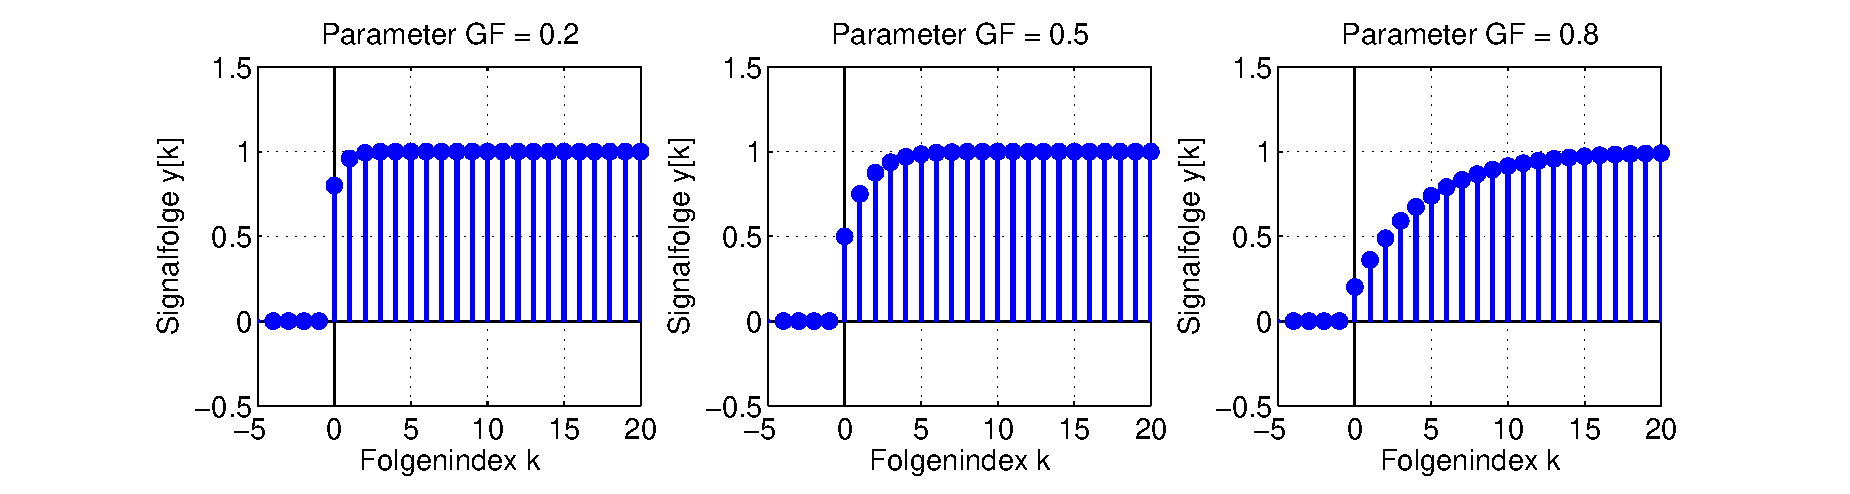
\includegraphics[width=1\textwidth]{Kapitel4/Bilder/image1.eps}}
  \caption{Ausgangssignal eines zeitdiskreten Tiefpass-Filters f\"{u}r einen Sprung am Eingang}
  \label{fig:RekursivTiefpass}
\end{figure}

\noindent Die Systemantworten erinnern an das Ausgangssignal eines Tiefpasses. Es wird sich zeigen, dass diese rekursive Form die digitale Approximation eines Tiefpasses erster Ordnung ist. \bigskip

\noindent
\colorbox{lightgray}{%
\arrayrulecolor{white}%
\renewcommand\arraystretch{0.6}%
\begin{tabular}{ wl{16.5cm} }
{\fontfamily{phv}\selectfont{Beispiel: Gleitender Mittelwert}}
\end{tabular}%
}\medskip

\noindent Zur Verringerung von St\"{o}reffekten kann der Mittelwert einiger aufeinanderfolgender Folgenwerte gebildet werden. Dieses Vorgehen wird als gleitende Mittelwertbildung bezeichnet. Zum Beispiel wird \"{u}ber die Gleichung

\begin{equation}\label{eq:fourtwo}
y\left[k\right]=\frac{1}{5} \cdot \left(u\left[k\right]+u\left[k-1\right]+u\left[k-2\right]+u\left[k-3\right]+u\left[k-4\right]\right)  
\end{equation}

\noindent ein gleitendes Mittelwertfilter mit 5 Abtastwerten beschrieben. Die Ausgangsfolge ist in diesem Fall nur von aktuellen und vergangenen Werten des Eingangssignals abh\"{a}ngig. Durch die Mittelwertbildung weist die Ausgangsfolge y[k] einerseits eine geringere Variation auf als die Eingangsfolge u[k]. Durch die Bildung des Mittelwertes von f\"{u}nf Abtastwerten erreicht das Signal andererseits sp\"{a}ter seinen Endwert. Beide Effekte sind in Bild \ref{fig:GleitenderMittelwert} verdeutlicht.

\begin{figure}[H]
  \centerline{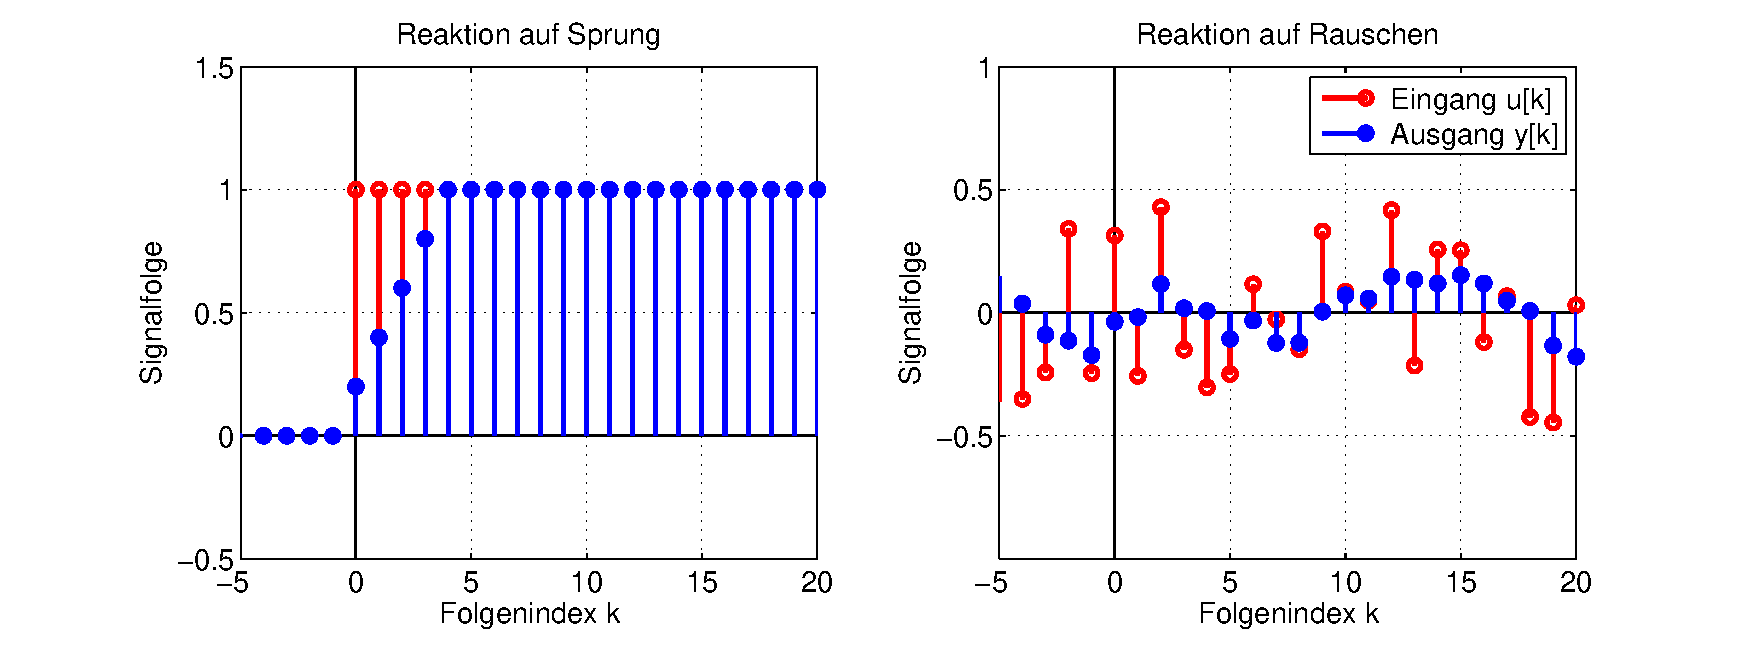
\includegraphics[width=1\textwidth]{Kapitel4/Bilder/image2.eps}}
  \caption{Ausgangssignal eines zeitdiskreten Systems mit gleitender Mittelung}
  \label{fig:GleitenderMittelwert}
\end{figure}

\InsertBoxL{0}{\includegraphics[scale=0.5]{Code.JPG}} 
\textcolor{white}{.}\newline
\noindent Im Online-Portal \textit{Systemtheorie Online} verdeutlicht die \textit{Applikation Signalabtastung und Signal-rekonstruktion} grafisch, welche Effekte durch Anti-Aliasing-Filter, reale Abtastung und reale Rekon-struktion entstehen.\newline   

\noindent Die beiden vorangegangenen Beispiele sind Algorithmen, die zum Beispiel als Programm in einem Controller implementiert werden k\"{o}nnen. Ein weiteres Anwendungsfeld f\"{u}r zeitdiskrete Systeme sind Switched-Capacitor-Schaltungen.\bigskip

\noindent
\colorbox{lightgray}{%
\arrayrulecolor{white}%
\renewcommand\arraystretch{0.6}%
\begin{tabular}{ wl{16.5cm} }
{\fontfamily{phv}\selectfont{Beispiel: Switched-Capacitor-Schaltung}}
\end{tabular}%
}\medskip

\noindent Bei der Integration von CMOS-Schaltungen ist es aufwendig und teuer, pr\"{a}zise und temperaturstabile Widerst\"{a}nde herzustellen. Die Herstellung von stabilen Kondensatoren ist dagegen vergleichsweise g\"{u}nstig. Deshalb werden in der CMOS-Technik Switched-Capacitor-Schaltungen verwendet. Als Beispiel zeigt Bild \ref{fig:SC_Filter} einen invertierenden Integrierer in Switched-Capacitor-Technik.

\begin{figure}[H]
  \centerline{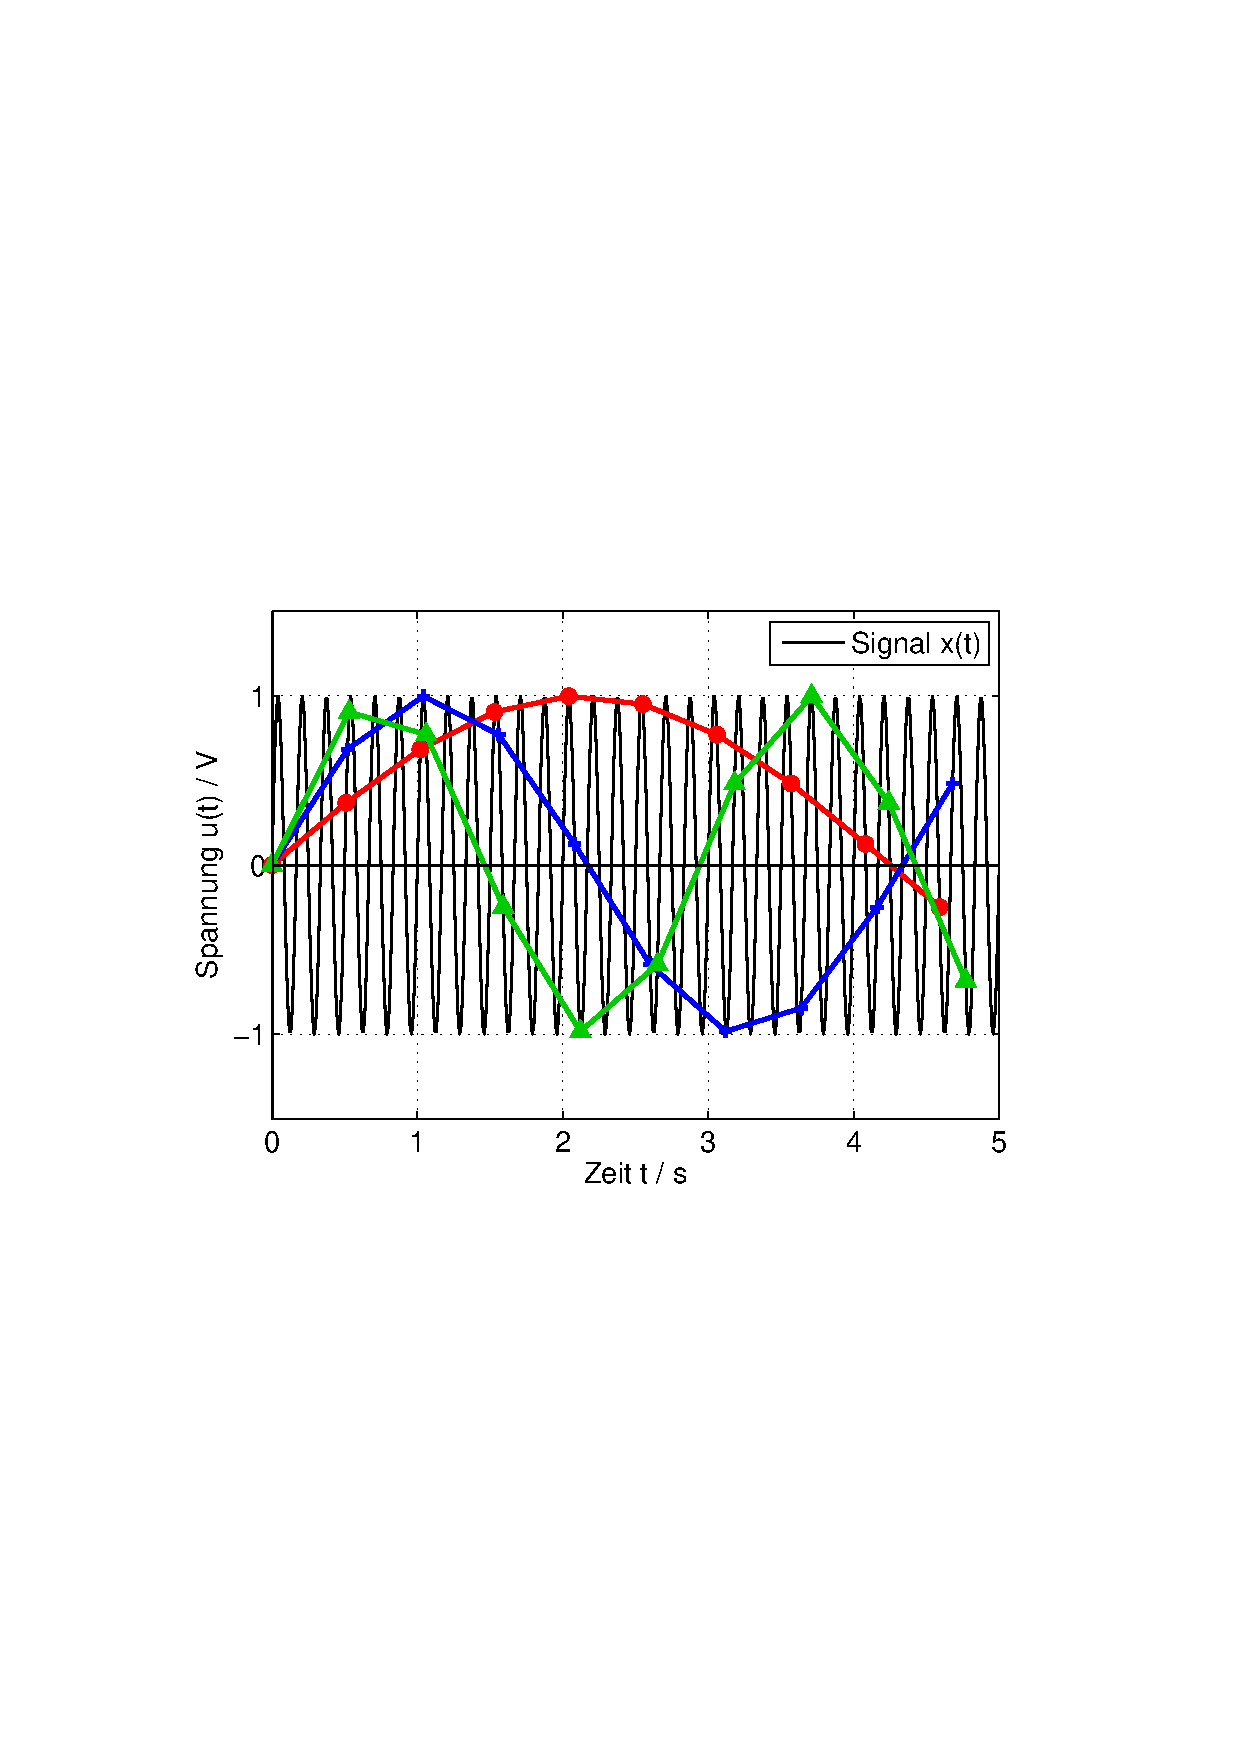
\includegraphics[width=0.35\textwidth]{Kapitel4/Bilder/image3.png}}
  \caption{Invertierender Integrierer in Switched-Capacitor-Technik}
  \label{fig:SC_Filter}
\end{figure}

\noindent Zu Beginn jeden Taktes wird der Kondensator C${}_{E}$ aufgeladen. Nach Umschalten des Schalters wird der Kondensator C${}_{E}$ mit dem Knoten A des Operationsverst\"{a}rkers verbunden, der auf Ground-Potential liegt. Der Kondensator wird dabei entladen. Da der Operationsverst\"{a}rker einen sehr gro{\ss}en Innenwiderstand besitzt, flie{\ss}t die Ladung nicht \"{u}ber den Operationsverst\"{a}rker ab, sondern zum Kondensator C${}_{A}$. Bei jedem Takt wird also dem Integrierer eine Ladung der Gr\"{o}{\ss}e q${}_{E}$[k] zugef\"{u}hrt.

\begin{equation}\label{eq:fourthree}
q_{E} \left[k\right]=u_{E} \left[k\right]\cdot C_{E}  
\end{equation}

\noindent Die aktuelle Ladung im Kondensator C${}_{A}$ betr\"{a}gt damit

\begin{equation}\label{eq:fourfour}
q_{A} \left[k\right]=u_{E} \left[k\right]\cdot C_{E} +q_{A} \left[k-1\right]=-u_{A} \left[k\right]\cdot C_{A}
\end{equation}

\noindent Die aktuelle Ladung q${}_{A}$[k] ergibt sich aus der Ladung im Takt zuvor und der dazukommenden Ladung. Die Ladung wird damit aufsummiert. Das aktuelle Ausgangssignal ergibt sich zu

\begin{equation}\label{eq:fourfive}
u_{A} [k]=-\frac{1}{C_{A} } \cdot q_{A} \left[k\right]=-\frac{1}{C_{A} } \cdot \left(u_{E} \left[k\right]\cdot C_{E} +q_{A} \left[k-1\right]\right)
\end{equation}

\noindent Wegen des Minuszeichens ist das System ein invertierender Summierer.\bigskip

\noindent Alle hier behandelten Beispiele f\"{u}hren auf eine Differenzengleichung, die in allgemeiner Form geschrieben werden kann als 

\begin{equation}\label{eq:foursix}
c_{0} \cdot y\left[k\right]+c_{1} \cdot y\left[k-1\right]+...+c_{n} \cdot y\left[k-N\right]=d_{0} \cdot u\left[k\right]+d_{1} \cdot u\left[k-1\right]+...+d_{L} \cdot u\left[k-L\right]
\end{equation}

\noindent Die L\"{o}sung dieser Differenzengleichung ist Gegenstand des Abschnitts 4.3. 

\subsubsection{Zeitdiskrete Approximation zeitkontinuierlicher Systeme}

\noindent Das Verhalten der Ein- und Ausgangsgr\"{o}{\ss}en eines realisierbaren, zeitkontinuierlichen LTI-Systems wird durch eine lineare Differentialgleichung N-ter Ordnung mit konstanten Koeffizienten beschrieben. Nach den Ausf\"{u}hrungen in Teil A dieser Buchreihe kann das System \"{u}ber Integrierer dargestellt werden. Beim \"{U}bergang von zeitkontinuierlichen zu zeitdiskreten Systemen kann die Integration nur approximiert werden. Eine Realisierungsm\"{o}glichkeit ist die Approximation mit einem Trapez. Bild \ref{fig:Differenzenquotient} verdeutlicht Ableitung die Integration und Approximation der Ableitung Integration grafisch.

\begin{figure}[H]
  \centerline{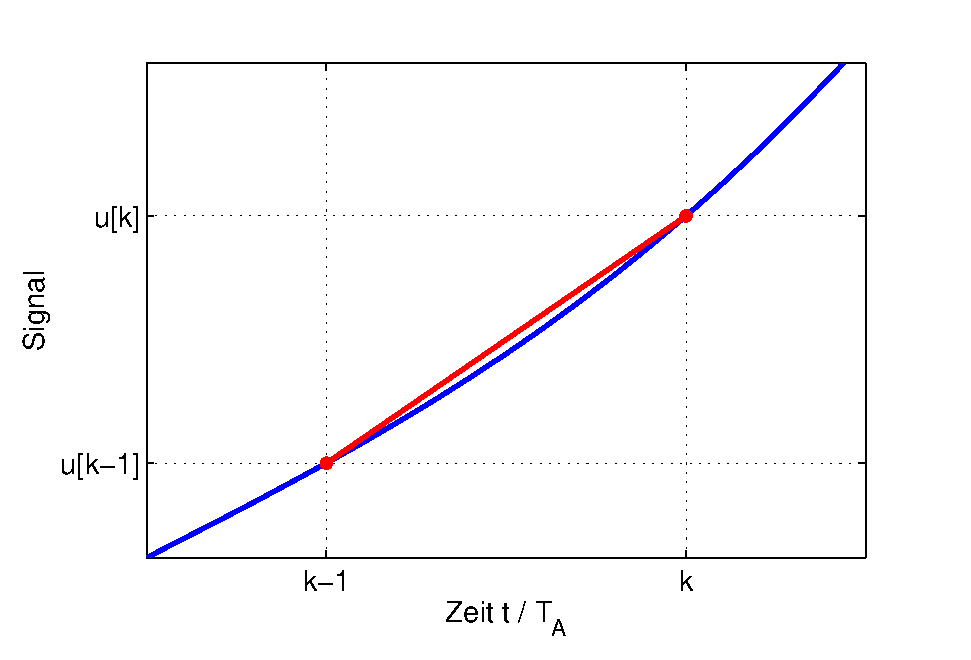
\includegraphics[width=0.5\textwidth]{Kapitel4/Bilder/image4.eps}}
  \caption{Approximation des Integrals eines zeitkontinuierlichen Signals durch ein Trapez}
  \label{fig:Differenzenquotient}
\end{figure}

\noindent Aus einem Vergleich der Fl\"{a}chen unter der Funktion u(t) ergibt sich der Ausdruck

\begin{equation}\label{eq:fourseven}
\int\limits _{\left(k-1\right)\cdot T_{A} }^{k\cdot T_{A} }u\left(t\right) {\rm \; }dt=\frac{1}{2} \cdot \left(u\left[k\right]+u\left[k-1\right]\right)\cdot T_{A}
\end{equation}

\noindent Die Approximation der Integration f\"{u}hrt zu der gewichteten Summe aufeinanderfolgender Abtastwerte, die mit dem Faktor T${}_{A}$ multipliziert wird. F\"{u}r Integrale h\"{o}herer Ordnung kann entsprechend verfahren werden. Es ergibt sich eine Summe von Folgenwerten, die jeweils um einen Abtastwert verschoben sind. Allgemein ist das aktuelle Ausgangssignal eine Funktion der vergangenen Ein- und Ausgangswerte und des aktuellen Eingangssignals.

\begin{equation}\label{eq:foureight}
y\left[k\right]=f\left(y\left[k-1\right],\, \, y\left[k-2\right],\, \, \, ...,\, \, u\left[k\right],\, \, u\left[k-1\right],\, \, u\left[k-2\right],\, \, ...\right)
\end{equation}

\noindent Die Beschreibung linearer, zeitinvarianter Systeme f\"{u}hrt zu linearen Differenzengleichungen mit konstanten Koeffizienten, die allgemein dargestellt werden k\"{o}nnen als

\begin{equation}\label{eq:fournine}
sum _{n=0}^{N}c_{n} \cdot y\left[k-n\right] =\sum _{l=0}^{L}d_{l} \cdot u\left[k-l\right]
\end{equation}

\noindent beziehungsweise mit c${}_{0}$ = 1

\begin{equation}\label{eq:fourten}
y\left[k\right]=\sum _{l=0}^{L}d_{l} \cdot u\left[k-l\right] -\sum _{n=1}^{N}c_{n} \cdot y\left[k-n\right]
\end{equation}

\noindent Die G\"{u}te der Approximation verbessert sich mit sinkender Abtastzeit T${}_{A}$. Allerdings ist die Abtastzeit aus der Anwendung vorgegeben. Auch der Signalverlauf hat einen Einfluss auf die Approximationsg\"{u}te. Nichtlineare Kurvenverl\"{a}ufe und hochfrequente Signalanteile wirken sich negativ auf die Approximationsg\"{u}te aus.\bigskip

\noindent
\colorbox{lightgray}{%
\arrayrulecolor{white}%
\renewcommand\arraystretch{0.6}%
\begin{tabular}{ wl{16.5cm} }
{\fontfamily{phv}\selectfont{Beispiel: RC-Tiefpass}}
\end{tabular}%
}\medskip

\noindent Bild \ref{fig:RCTiefpass} zeigt einen RC-Tiefpass mit Spannungsquelle u${}_{E}$, Widerstand R und Kapazit\"{a}t C.

\begin{figure}[H]
  \centerline{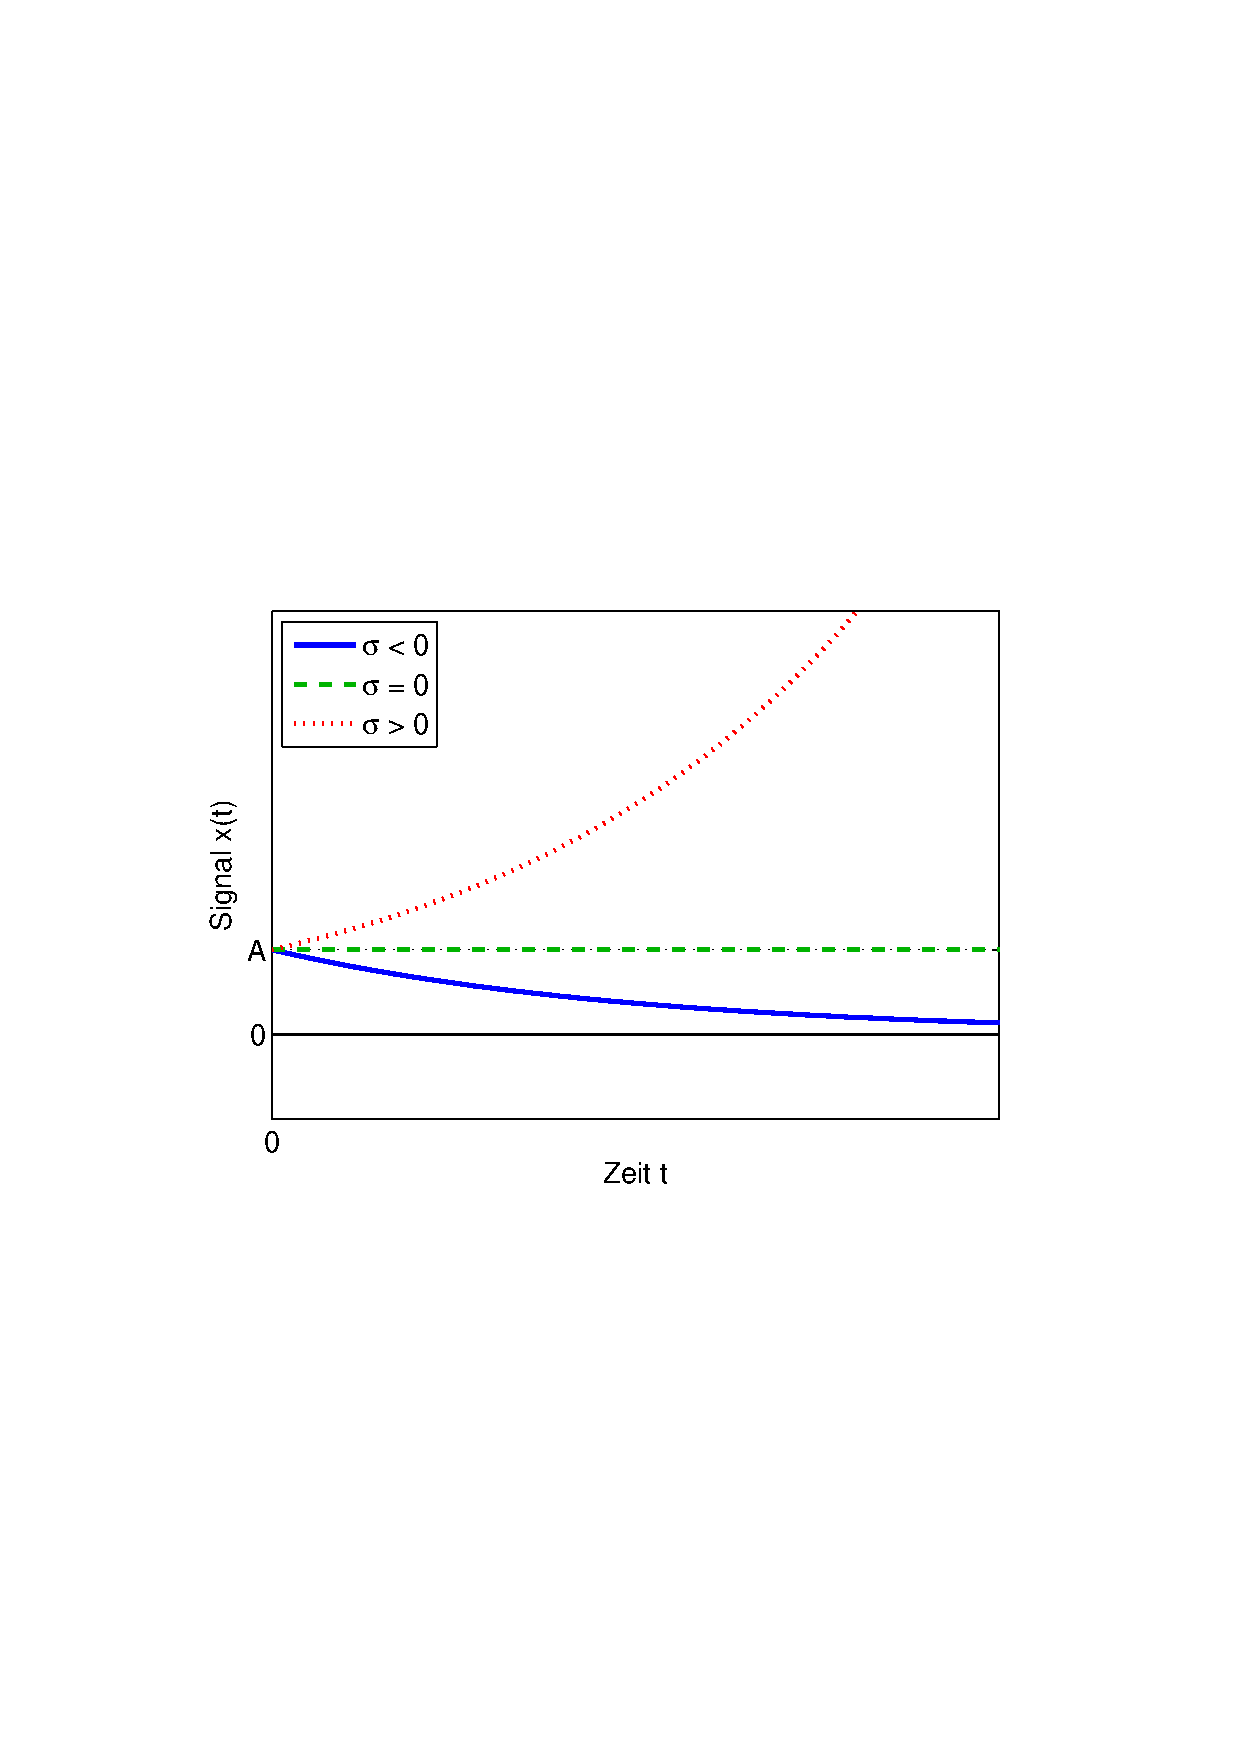
\includegraphics[width=0.35\textwidth]{Kapitel4/Bilder/image5.png}}
  \caption{RC-Tiefpass}
  \label{fig:RCTiefpass}
\end{figure}

\noindent Die zugeh\"{o}rige lineare Differentialgleichung f\"{u}r die Ausgangsspannung u${}_{A}$(t) lautet:

\begin{equation}\label{eq:foureleven}
u_{A} \left(t\right)+R\cdot C\cdot \frac{du_{A} }{dt} =u_{E} \left(t\right)
\end{equation}

\noindent Eine Integration der Differentialgleichung f\"{u}hrt bei zeitdiskreten Integrationsgrenzen zu

\begin{equation}\label{eq:fourtwelve}
\int\limits _{\left(k-1\right)\cdot T_{A} }^{k\cdot T_{A} }u_{A} \left(t\right){\rm \; } dt+R\cdot C\cdot \left(u_{A} \left(k\cdot T_{A} \right)-u_{A} \left(\left(k-1\right)\cdot T_{A} \right)\right)=\int\limits _{\left(k-1\right)\cdot T_{A} }^{k\cdot T_{A} }u_{A} \left(t\right){\rm \; } dt
\end{equation}

\noindent Mit den Signalen

\begin{equation}\label{eq:fourthirteen}
u_{E} \left(k\cdot T_{A} \right)=u_{E} \left[k\right]
\end{equation}

\noindent und

\begin{equation}\label{eq:fourfourteen}
u_{A} \left(k\cdot T_{A} \right)=u_{A} \left[k\right]
\end{equation}

\noindent und einer Approximation der Integrale \"{u}ber die Trapezregel ergibt sich

\begin{equation}\label{eq:fourfiveteen}
\frac{1}{2} \cdot \left(u_{A} \left[k\right]+u_{A} \left[k-1\right]\right)\cdot T_{A} +R\cdot C\cdot \left(u_{A} \left[k\right]-u_{A} \left[k-1\right]\right)=\frac{1}{2} \cdot \left(u_{E} \left[k\right]+u_{E} \left[k-1\right]\right)\cdot T_{A}
\end{equation}

\noindent Zur Berechnung des aktuellen Ausgangssignals wird die Gleichung ausmultipliziert und nach u${}_{A}$[k] aufgel\"{o}st.

\begin{equation}\label{eq:foursixteen}
u_{A} \left[k\right]=\frac{T_{A} \cdot u_{E} \left[k\right]+T_{A} \cdot u_{E} \left[k-1\right]-T_{A} \cdot u_{A} \left[k-1\right]+2\cdot R\cdot C\cdot u_{A} \left[k-1\right]}{T_{A} +2\cdot R\cdot C} 
\end{equation}

\noindent Die aktuelle Ausgangsspannung u${}_{A}$[k] berechnet sich aus dem aktuellen und einem vergangenen Wert der Eingangsspannung u${}_{E}$[k] und einem vergangenen Wert der Ausgangsspannung u${}_{A}$[k]. Bild \ref{fig:RCEinschwingen} zeigt den Vergleich zwischen dem zeitkontinuierlichen und dem zeitdiskreten System bei unterschiedlichen Abtastzeiten.

\begin{figure}[H]
  \centerline{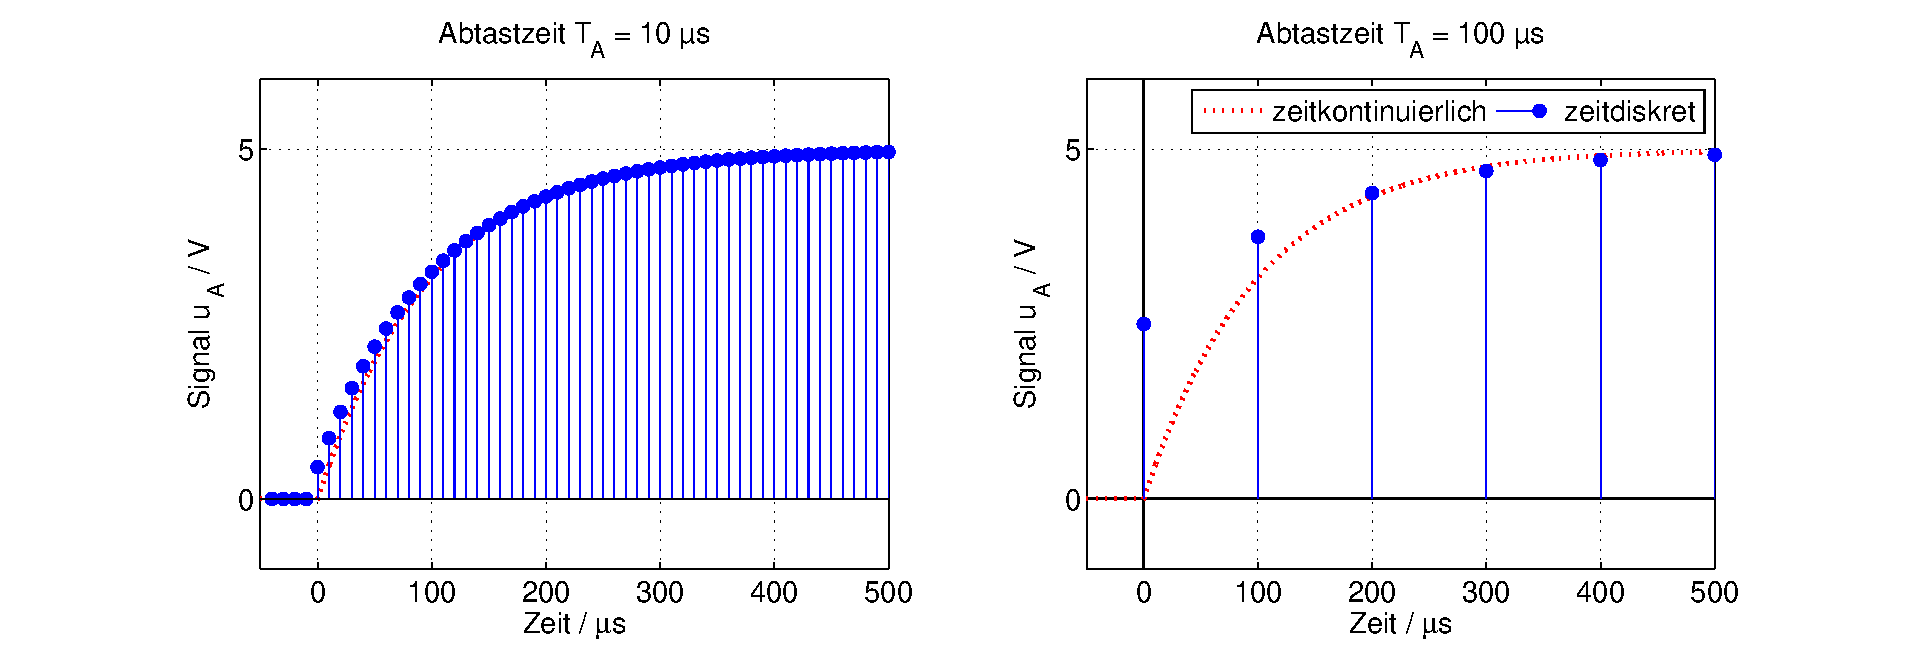
\includegraphics[width=1\textwidth]{Kapitel4/Bilder/image6.eps}}
  \caption{Vergleich zwischen zeitkontinuierlicher und zeitdiskreter Realisierung eines Tiefpasses (R$\cdot$C = 100 µs)}
  \label{fig:RCEinschwingen}
\end{figure}

\noindent Die Abtastzeit von T${}_{A}$ = 10 µs ist deutlich kleiner als die Zeitkonstante des Systems mit T = 100 µs. Aus diesem Grund ist die Approximationsg\"{u}te im links dargestellten Fall hoch. Die im rechten Bildteil diskutierte Abtastzeit von T${}_{A}$ = 100 µs entspricht der Zeitkonstante des Systems. Aus diesem Grund ist die Approximation der Ableitung mit einem Differenzenquotienten unzureichend, die Approximationsg\"{u}te ist deutlich schlechter als bei einer Abtastzeit von T${}_{A}$ = 10 µs. Das Beispiel zeigt, dass zeitkontinuierliche Systeme zeitdiskret nachgebildet werden k\"{o}nnen. Die lineare Differentialgleichung erster Ordnung 

\begin{equation}\label{eq:fourseventeen}
u_{A} \left(t\right)+R\cdot C\cdot \frac{du_{A} }{dt} =u_{E} \left(t\right)
\end{equation}

\noindent geht dabei \"{u}ber in eine lineare Differenzengleichung erster Ordnung.

\begin{equation}\label{eq:foureighteen}
\left(T_{A} +2\cdot R\cdot C\right)\cdot u_{A} \left[k\right]+\left(T_{A} -2\cdot R\cdot C\right)\cdot u_{A} \left[k-1\right]=T_{A} \cdot u_{E} \left[k\right]+T_{A} \cdot u_{E} \left[k-1\right]
\end{equation}

\noindent Die hier diskutierten Beispiele f\"{u}hren auf lineare Differenzengleichungen mit konstanten Koeffizienten.

\begin{equation}\label{eq:fournineteen}
c_{0} \cdot y\left[k\right]+c_{1} \cdot y\left[k-1\right]+...+c_{n} \cdot y\left[k-N\right]=d_{0} \cdot u\left[k\right]+d_{1} \cdot u\left[k-1\right]+...+d_{L} \cdot u\left[k-L\right]
\end{equation}

\noindent Im Folgenden werden die Eigenschaften von Systemen diskutiert, die sich mit dieser Art von Differenzengleichungen beschreiben lassen.

\clearpage

\subsection{Grundlegende Systemeigenschaften}\label{threetwo}

\noindent Im Abschnitt \ref{sfourone} werden unterschiedliche Systeme beschrieben. Die Beschreibung f\"{u}hrt zu linearen Differenzengleichungen mit konstanten Koeffizienten. In diesem Abschnitt werden grundlegende Eigenschaften von Systemen diskutiert. Sie entsprechen den Eigenschaften linearer, zeitinvarianter Systeme im zeitkontinuierlichen Bereich. Es wird sich zeigen, dass lineare Differenzengleichungen mit konstanten Koeffizienten zeitdiskrete, lineare, zeitinvariante Systeme (LTI-Systeme) beschreiben.

\subsubsection{Linearität}

\noindent F\"{u}r den Linearit\"{a}tsnachweis eines Systems m\"{u}ssen die Systemantworten y${}_{1}$[k] und y${}_{2}$[k] auf die Eingangsfolgen u${}_{1}$[k] und u${}_{2}$[k] bekannt sein. Ein System ist linear, wenn es auf eine Linearkombination von Eingangssignalen 

\begin{equation}\label{eq:fourtwenty}
u\left[k\right]=\nu _{1} \cdot u_{1} \left[k\right]+\nu _{2} \cdot u_{2} \left[k\right]
\end{equation}

\noindent mit derselben Linearkombination der entsprechenden Ausgangssignale reagiert. 

\begin{equation}\label{eq:fourtwentyone}
u\left[k\right]=\nu _{1} \cdot u_{1} \left[k\right]+\nu _{2} \cdot u_{2} \left[k\right]
\end{equation}

\noindent Der Nachweis erfolgt \"{u}ber Einsetzen der Gleichungen in die Differenzengleichung.\bigskip

\noindent
\colorbox{lightgray}{%
\arrayrulecolor{white}%
\renewcommand\arraystretch{0.6}%
\begin{tabular}{ wl{16.5cm} }
{\fontfamily{phv}\selectfont{Beispiel: Linearit\"{a}t eines r\"{u}ckgekoppelten Systems}}
\end{tabular}%
}\medskip

\noindent Das Filter mit der Differenzengleichung 

\begin{equation}\label{eq:fourtwentytwo}
y\left[k\right]=\left(1-GF\right)\cdot u\left[k\right]+GF\cdot y\left[k-1\right]
\end{equation}

\noindent soll auf Linearit\"{a}t untersucht werden. Die Systemantworten y${}_{1}$[k] und y${}_{2}$[k] berechnen sich mit der Differenzengleichung zu

\begin{equation}\label{eq:fourtwentythree}
y_{1} \left[k\right]=\left(1-GF\right)\cdot u_{1} \left[k\right]+GF\cdot y_{1} \left[k-1\right]
\end{equation}

\noindent beziehungsweise

\begin{equation}\label{eq:fourtwentyfour}
y_{2} \left[k\right]=\left(1-GF\right)\cdot u_{2} \left[k\right]+GF\cdot y_{2} \left[k-1\right]
\end{equation}

\noindent Wird das System mit der oben beschriebenen Linearkombination angeregt, ergibt sich das Ausgangssignal y[k] aus derselben Linearkombination wie die Eingangssignale.

\begin{equation}\label{eq:fourtwentyfive}
\begin{split}
y\left[k\right] & = \left(1-GF\right)\cdot u\left[k\right]+GF\cdot y\left[k-1\right] \\ 
& = \left(1-GF\right)\cdot \left(\nu _{1} \cdot u_{1} \left[k\right]+\nu _{2} \cdot u_{2} \left[k\right]\right)+GF\cdot \left(\nu _{1} \cdot y_{1} \left[k-1\right]+\nu _{2} \cdot y_{2} \left[k-1\right]\right) \\ 
& = \left(1-GF\right)\cdot \nu _{1} \cdot u_{1} \left[k\right]+\left(1-GF\right)\cdot \nu _{2} \cdot u_{2} \left[k\right]+GF\cdot \nu _{1} \cdot y_{1} \left[k-1\right]+GF\cdot \nu _{2} \cdot y_{2} \left[k-1\right] \\ 
& = nu _{1} \cdot \left(1-GF\right)\cdot u_{1} \left[k\right]+\nu _{1} \cdot GF\cdot y_{1} \left[k-1\right]+\nu _{2} \cdot \left(1-GF\right)\cdot u_{2} \left[k\right]+\nu _{2} \cdot GF\cdot y_{2} \left[k-1\right] \\ 
& = \nu _{1} \cdot y_{1} \left[k\right]+\nu _{2} \cdot y_{2} \left[k\right]
\end{split}
\end{equation}

\noindent Bild \ref{fig:RekursivTiefpassLinearitaet} zeigt Ein- und Ausgangssignale eines linearen Systems, das mit den Signalen u${}_{1}$[k], u${}_{2}$[k] und u[k] = u${}_{1}$[k] + u${}_{2}$[k] angeregt wird. 

\begin{figure}[H]
  \centerline{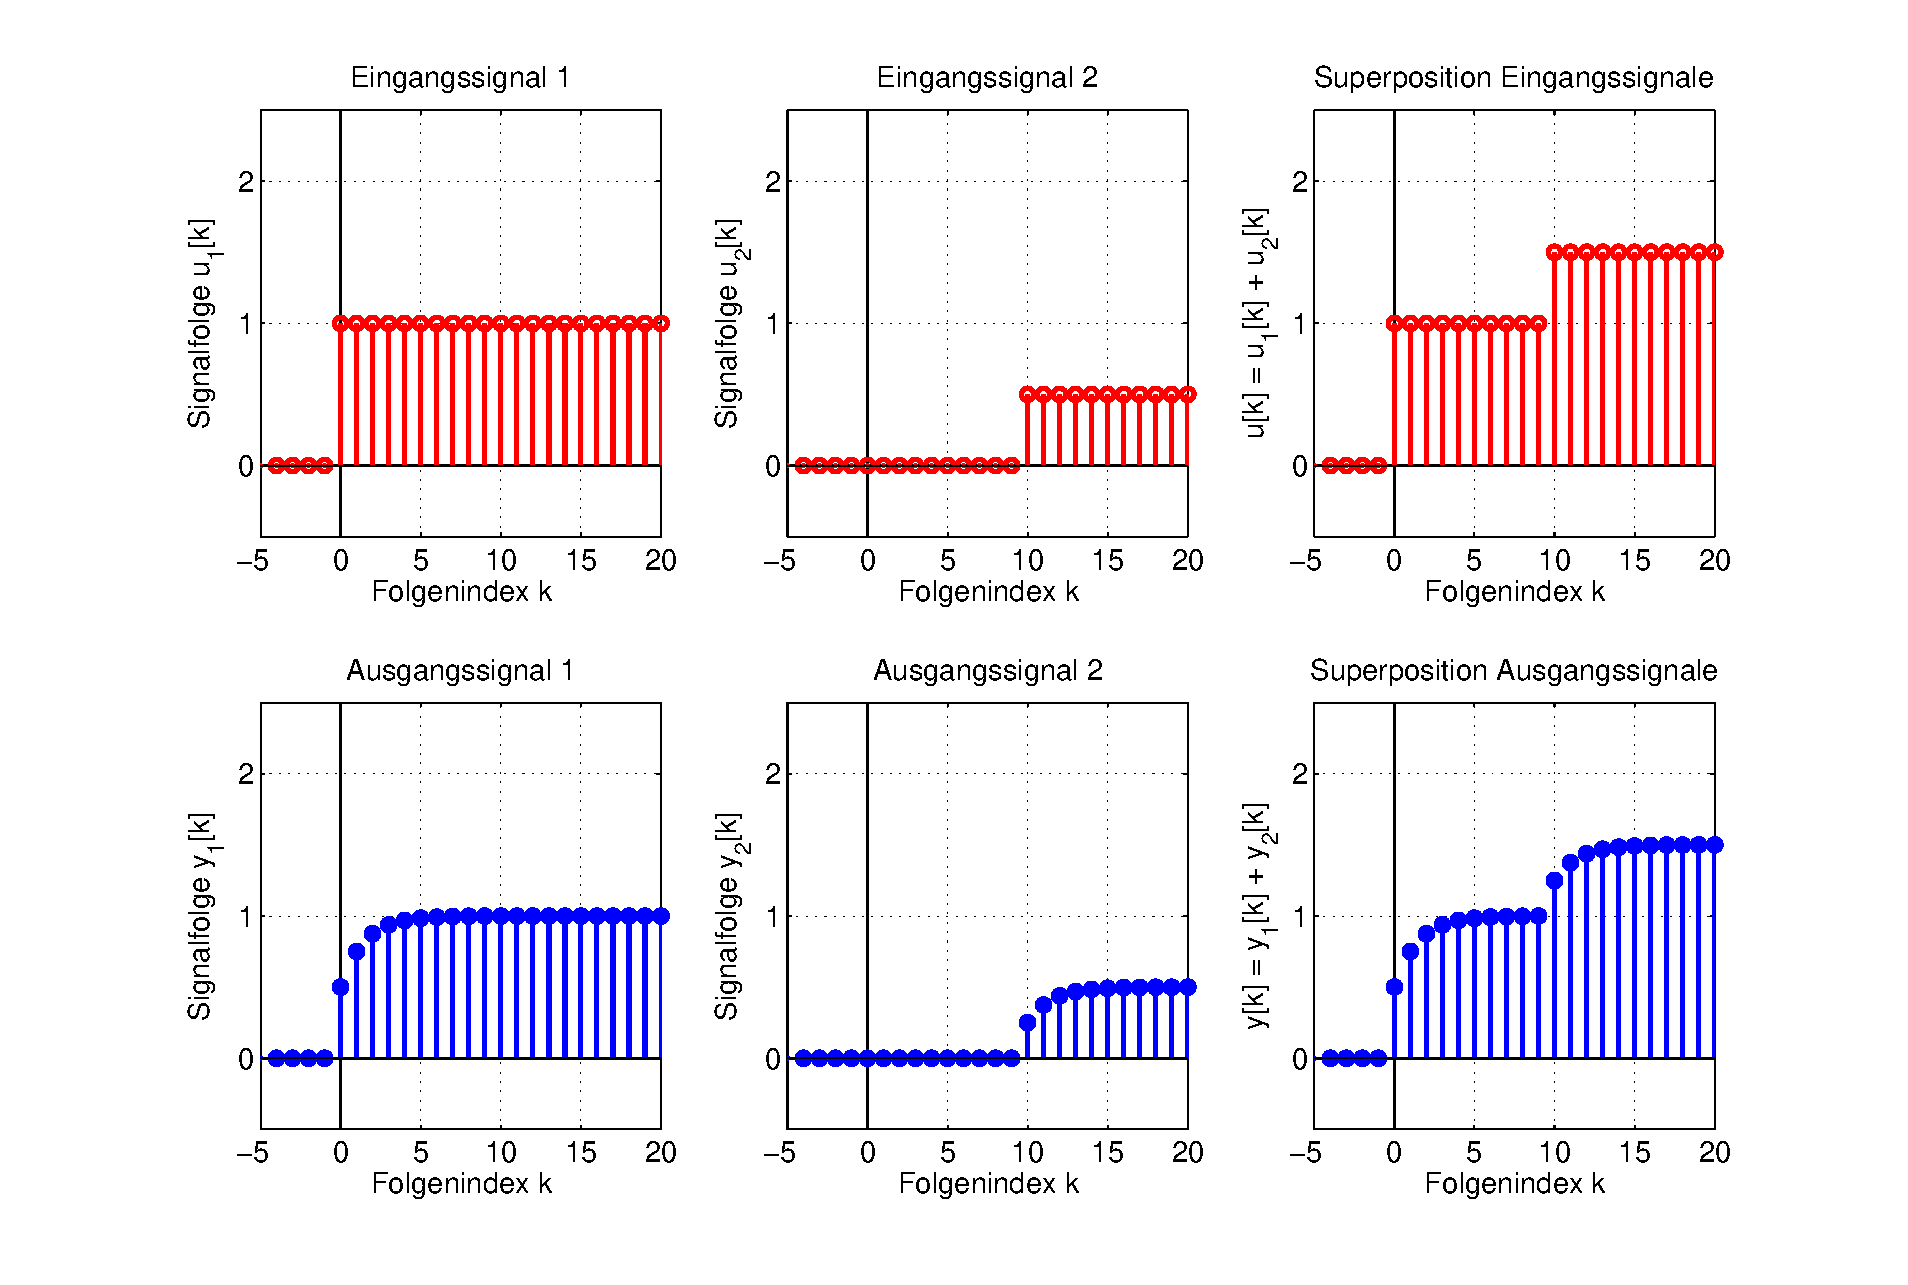
\includegraphics[width=1\textwidth]{Kapitel4/Bilder/image7.eps}}
  \caption{Reaktion eines linearen Systems auf die Anregung mit einer Linearkombination von Signalen}
  \label{fig:RekursivTiefpassLinearitaet}
\end{figure}

\noindent Auch das Ausgangssignal y[k] setzt sich aus der Summe der Ausgangsignale y${}_{1}$[k] und y${}_{2}$[k] zusammen.\bigskip

\noindent Die Linearit\"{a}t des Systems kann auch daran abgelesen werden, dass alle Folgen nur in linearen Summen auftreten. Keine der Folgen besitzt eine Potenz ungleich 1 oder tritt als Produkt von Folgen auf. 

\subsubsection{Zeitvarianz}

\noindent Ein System reagiert auf ein Eingangssignal u[k] mit einer Systemantwort y[k]. Ist das System zeitinvariant, so reagiert das System auf das verz\"{o}gerte Eingangssignal u[k - k${}_{0}$] mit dem Ausgangsignal y[k - k${}_{0}$]. Zeitinvariante Systeme reagieren also unabh\"{a}ngig vom Startzeitpunkt der Beobachtung auf gleiche Eingangssignale mit gleichen Ausgangssignalen.\bigskip

\noindent
\colorbox{lightgray}{%
\arrayrulecolor{white}%
\renewcommand\arraystretch{0.6}%
\begin{tabular}{ wl{16.5cm} }
{\fontfamily{phv}\selectfont{Beispiel: Zeitinvarianz eines r\"{u}ckgekoppelten Systems}}
\end{tabular}%
}\medskip

\noindent Das Filter mit der Differenzengleichung 

\begin{equation}\label{eq:fourtwentysix}
y\left[k\right]=\left(1-GF\right)\cdot u\left[k\right]+GF\cdot y\left[k-1\right]
\end{equation}

\noindent soll auf Zeitinvarianz untersucht werden. Dazu werden alle Ausdr\"{u}cke k durch k -- k${}_{0}$ ersetzt. Es ergibt sich die Differenzengleichung

\begin{equation}\label{eq:fourtwentyseven}
y\left[k-k_{0} \right]=\left(1-GF\right)\cdot u\left[k-k_{0} \right]+GF\cdot y\left[k-k_{0} -1\right]
\end{equation}

\noindent Wird das Eingangssignal um k${}_{0}$ verschoben, wird auch das Ausgangsignal um k${}_{0}$ verschoben.

\begin{figure}[H]
  \centerline{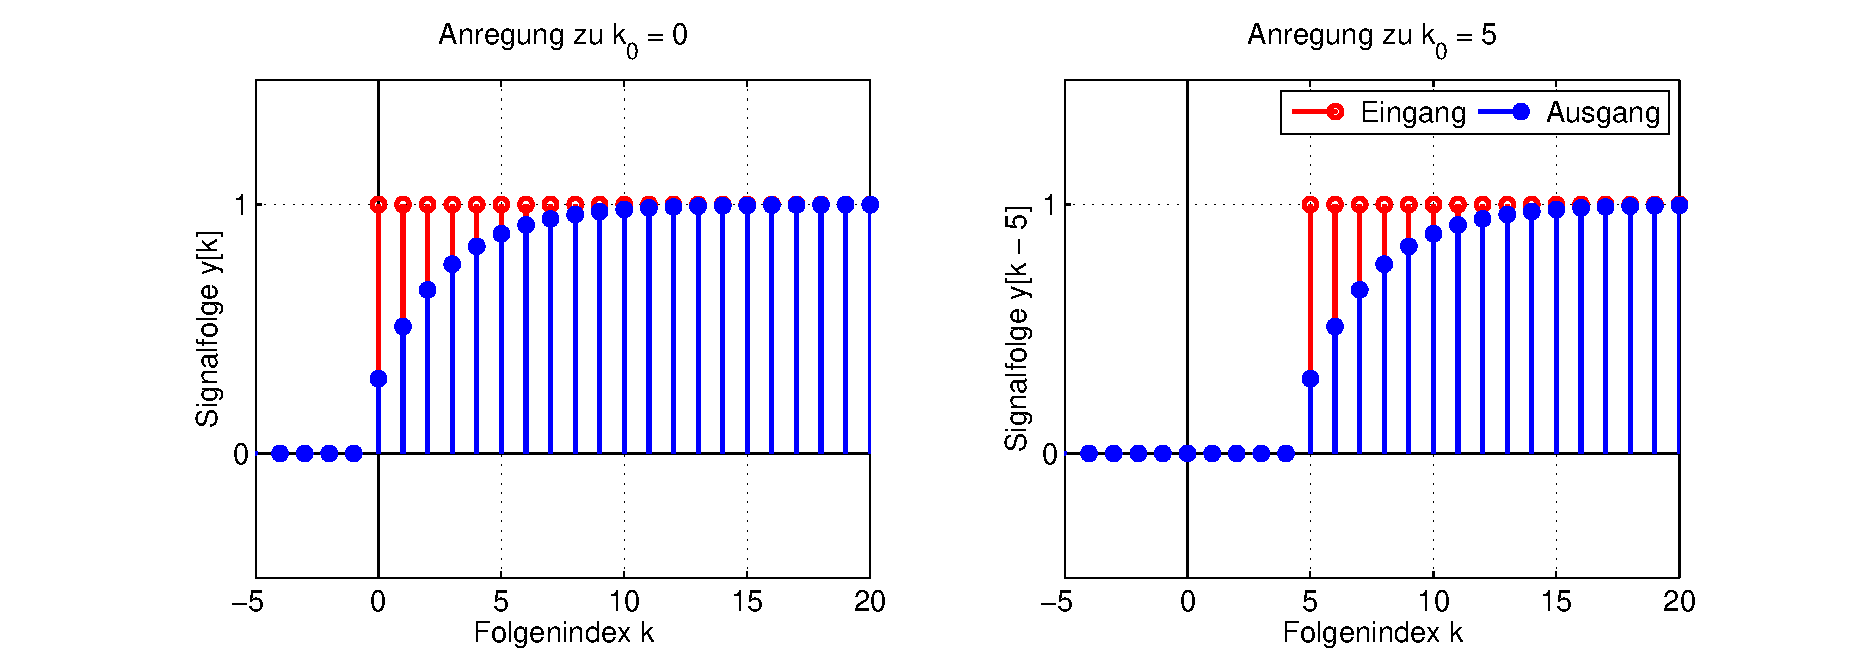
\includegraphics[width=1\textwidth]{Kapitel4/Bilder/image8.eps}}
  \caption{Reaktion eines zeitinvarianten Systems auf die Anregung mit zeitverschobenen Signalen}
  \label{fig:RekursivTiefpassZeitinvarianz}
\end{figure}

\noindent Es kann gezeigt werden, dass zeitinvariante Systeme Differenzengleichungen mit konstanten Koeffizienten aufweisen. \"{A}ndern sich die Koeffizienten der Differenzengleichung mit dem Folgenindex k, ist das System zeitvariant. 

\subsubsection{Lineare, zeitinvariante Systeme (LTI-Systeme)}\label{fourtwothree}

\noindent Die Darstellungen in diesem Skript beschr\"{a}nken sich bis auf wenige Ausnahmen auf Systeme, die linear und zeitinvariant sind und als LTI-Systeme bezeichnet werden. F\"{u}r LTI-Systeme sind besonders anschauliche und einfach zu interpretierende L\"{o}sungs- und Interpretationsmethoden im Zeit-, Bild- und Frequenzbereich vorhanden. Sie entsprechen sinngem\"{a}{\ss} den Methoden zeitkontinuierlicher Systeme.\medskip


\centerline{\includegraphics[width=0.6\textwidth]{Kapitel4/Bilder/image3.11.png}}
{\fontfamily{phv}\selectfont{\centerline{Bild 3.11: Lineares zeitinvariantes System} }}\bigskip

\noindent Systeme, die mit einer linearen Differenzengleichung mit konstanten Koeffizienten beschrieben werden k\"{o}nnen, erf\"{u}llen die Bedingungen nach Linearit\"{a}t und Zeitinvarianz. Ausgehend von der Differenzengleichung

\begin{equation}\label{eq:fourtwentyeight}
\sum _{n=0}^{N}c_{n} \cdot y\left[k-n\right] =\sum _{l=0}^{L}d_{l} \cdot u\left[k-l\right] 
\end{equation}

\noindent werden die Eigenschaften der Linearit\"{a}t und Zeitinvarianz hergeleitet.\bigskip

{\fontfamily{phv}\selectfont
\noindent\textbf{Linearität}} \smallskip

\noindent Ausgangspunkt f\"{u}r den Beweis der Linearit\"{a}t sind zwei Signalkombinationen u${}_{1}$[k] und y${}_{1}$[k] sowie u${}_{2}$[k] und y${}_{2}$[k], f\"{u}r die gilt

\begin{equation}\label{eq:fourtwentynine}
\sum _{n=0}^{N}c_{n} \cdot y_{1} \left[k-n\right] =\sum _{l=0}^{L}d_{l} \cdot u_{1} \left[k-l\right]
\end{equation}

\begin{equation}\label{eq:fourthirty}
\sum _{n=0}^{N}c_{n} \cdot y_{2} \left[k-n\right] =\sum _{l=0}^{L}d_{l} \cdot u_{2} \left[k-l\right] 
\end{equation}

\noindent F\"{u}r eine beliebige Linearkombination 

\begin{equation}\label{eq:fourthirtyone}
u\left[k\right]=\nu _{1} \cdot u_{1} \left[k\right]+\nu _{2} \cdot u_{2} \left[k\right]
\end{equation}

\noindent gilt dann die Gleichung

\begin{equation}\label{eq:fourthirtytwo}
\begin{split}
\sum _{l=0}^{L}d_{l} \cdot u\left[k-l\right]  & = \sum _{l=0}^{L}d_{l} \cdot \nu _{1} \cdot u_{1} \left[k-l\right]+d_{l} \cdot \nu _{2} \cdot u_{2} \left[k-l\right]  \\ 
& = \nu _{1} \cdot \sum _{l=0}^{L}d_{l} \cdot u_{1} \left[k-l\right]+d_{l} + \nu_{2}  \cdot \sum _{l=0}^{L}d_{l} \cdot  u_{2}\left[k-l\right] 
\end{split}
\end{equation}

\noindent F\"{u}r jede der beiden Summen kann der Ausdruck aus \eqref{eq:fourtwentynine} beziehungsweise \eqref{eq:fourthirty} eingesetzt werden, und es ergibt sich

\begin{equation}\label{eq:fourthirtythree}
\begin{split}
\sum _{l=0}^{L}d_{l} \cdot u\left[k-l\right] & = \nu _{1} \cdot \sum _{n=0}^{N}c_{n} \cdot y_{1} \left[k-n\right] +\nu _{2} \cdot \sum _{n=0}^{N}c_{n} \cdot y_{2} \left[k-n\right] \\
& = \sum _{n=0}^{N}c_{n} c_{n} \cdot ( \nu_{1} \cdot y_{1} [k-n] + \nu_{2} \cdot y_{2} [k-n]) = \sum _{n=0}^{N}c_{n} c_{n} \cdot y[k-n]
\end{split}
\end{equation}

\noindent Eine Linearkombination von Eingangssignalen f\"{u}hrt damit zu der identischen Linearkombination von Ausgangssignalen, sodass das System ein lineares System ist.\bigskip

{\fontfamily{phv}\selectfont
\noindent\textbf{Zeitinvarianz}} \smallskip

\noindent Wie oben bereits beschrieben sind lineare Differenzengleichungen mit konstanten Koeffizienten stets zeitinvariant. Wird in der Differenzengleichung

\begin{equation}\label{eq:fourthirtyfour}
\sum _{n=0}^{N}c_{n} \cdot y\left[k-n\right] =\sum _{l=0}^{L}d_{l} \cdot u\left[k-l\right]
\end{equation}

\noindent der Folgenindex sowohl bei Eingangs- als auch Ausgangssignalen um k${}_{0}$ verschoben, bleibt die Differenzengleichung weiter g\"{u}ltig.

\begin{equation}\label{eq:fourthirtyfive}
\sum _{n=0}^{N}c_{n} \cdot y\left[k-k_{0} -n\right] =\sum _{l=0}^{L}d_{l} \cdot u\left[k-k_{0} -l\right]
\end{equation}

{\fontfamily{phv}\selectfont
\noindent\textbf{Kausalit\"{a}t}} \smallskip

\noindent Wesentliche Voraussetzung f\"{u}r die Realisierbarkeit eines Systems ist die Forderung, dass die Werte der Ausgangssignale zu einem gegebenen Zeitpunkt nur von Werten der Eingangssignale zu diesem oder einem fr\"{u}heren Zeitpunkt abh\"{a}ngen, nicht jedoch etwa von zuk\"{u}nftigen Werten. Dieses Verhalten wird f\"{u}r zeitkontinuierliche Systeme als die Eigenschaft der Kausalit\"{a}t eines Systems definiert, die auch im diskreten Fall wesentlich ist. Liegt eine Systembeschreibung \"{u}ber eine Differenzengleichung vor, kann die Kausalit\"{a}t direkt bewertet werden. 

\begin{equation}\label{eq:fourthirtysix}
\sum _{n=0}^{N}c_{n} \cdot y\left[k-n\right] =\sum _{l=0}^{L}d_{l} \cdot u\left[k-l\right]
\end{equation}

\noindent Ist der Koeffizient c${}_{0}$ $\neq$ 0, kann ohne Beschr\"{a}nkung der Allgemeinheit die Annahme c${}_{0}$ = 1 getroffen werden. Ist das nicht der Fall, wird die Gleichung durch c${}_{0}$ dividiert. Mit dieser Annahme kann die Differenzengleichung nach y[k] aufgel\"{o}st werden, und es ergibt sich

\begin{equation}\label{eq:fourthirtyseven}
y\left[k\right]=\sum _{l=0}^{L}d_{l} \cdot u\left[k-l\right] -\sum _{n=1}^{N}c_{n} \cdot y\left[k-n\right] 
\end{equation}

\noindent Da alle Indizes m l und n gr\"{o}{\ss}er gleich null sind, ist ein System, das durch eine lineare Differenzengleichung der Form aus Gleichung \eqref{eq:fourthirtyseven} beschrieben werden kann, ein kausales System. Ist in der Differenzengleichung \eqref{eq:fourthirtysix} der Koeffizient c${}_{0}$ = 0, kann nicht nach y[k] aufgel\"{o}st werden. Wird nach y[k - 1] aufgel\"{o}st, ergibt sich die Gleichung

\begin{equation}\label{eq:fourthirtyeight}
y\left[k-1\right]=\frac{1}{c_{1} } \cdot \left(\sum _{l=0}^{L}d_{l} \cdot u\left[k-l\right] -\sum _{n=2}^{N}c_{n} \cdot y\left[k-n\right] \right)
\end{equation}

\noindent Damit ist der Ausgangswert y[k - 1] von dem zuk\"{u}nftigen Eingangswert u[k] abh\"{a}ngig. Das System ist demnach f\"{u}r c${}_{0}$ = 0 nicht kausal.\bigskip 

\noindent Durch die Kausalit\"{a}tsforderung sind einige Systembetrachtungen der digitalen Signalverarbeitung aufwendig. Daher werden im Folgenden aus Vereinfachungsgr\"{u}nden auch nicht-kausale Systeme betrachtet. Diese Systeme k\"{o}nnen aber vielfach durch eine Verschiebung kausal und damit realisierbar gemacht werden.\bigskip

\noindent
\colorbox{lightgray}{%
\arrayrulecolor{white}%
\renewcommand\arraystretch{0.6}%
\begin{tabular}{ wl{16.5cm} }
{\fontfamily{phv}\selectfont{Beispiel: Kausalit\"{a}t des gleitenden Mittelwertes}}
\end{tabular}%
}\medskip

\noindent Bei der Beschreibung zeitdiskreter Systeme wird der gleitende Mittelwert vorgestellt. Er hat die Differenzengleichung 

\begin{equation}\label{eq:fourthirtynine}
y_{1} \left[k\right]=\frac{1}{5} \cdot \left(u\left[k\right]+u\left[k-1\right]+u\left[k-2\right]+u\left[k-3\right]+u\left[k-4\right]\right)
\end{equation}

\noindent Weil das Ausgangssignal y[k] nur von aktuellen und vergangenen Eingangswerten abh\"{a}ngt, ist das System kausal. Es weist aber eine zeitliche Verz\"{o}gerung auf, die bei der Berechnung von Frequenzg\"{a}ngen noch dargestellt wird. Ein System mit der Differenzengleichung

\begin{equation}\label{eq:fourfourty}
y_{2} \left[k\right]=\frac{1}{5} \cdot \left(u\left[k+2\right]+u\left[k+1\right]+u\left[k\right]+u\left[k-1\right]+u\left[k-2\right]\right)
\end{equation}

\noindent ist nicht mehr kausal, weist aber - wie sp\"{a}ter gezeigt wird - keine zeitliche Verz\"{o}gerung auf. Oft werden in der Datenverarbeitung erst alle Messwerte aufgenommen und anschlie{\ss}end ausgewertet. In diesem Fall liegen auch zuk\"{u}nftige Werte vor. Die Kausalit\"{a}t von Systemen ist in diesem Fall nicht zwingend erforderlich. Bild \ref{fig:GleitenderMittelwertKausal} stellt die Sprungantwort eines kausalen und eines nicht kausalen Systems zur Berechnung eines gleitenden Mittelwertes dar.

\begin{figure}[H]
  \centerline{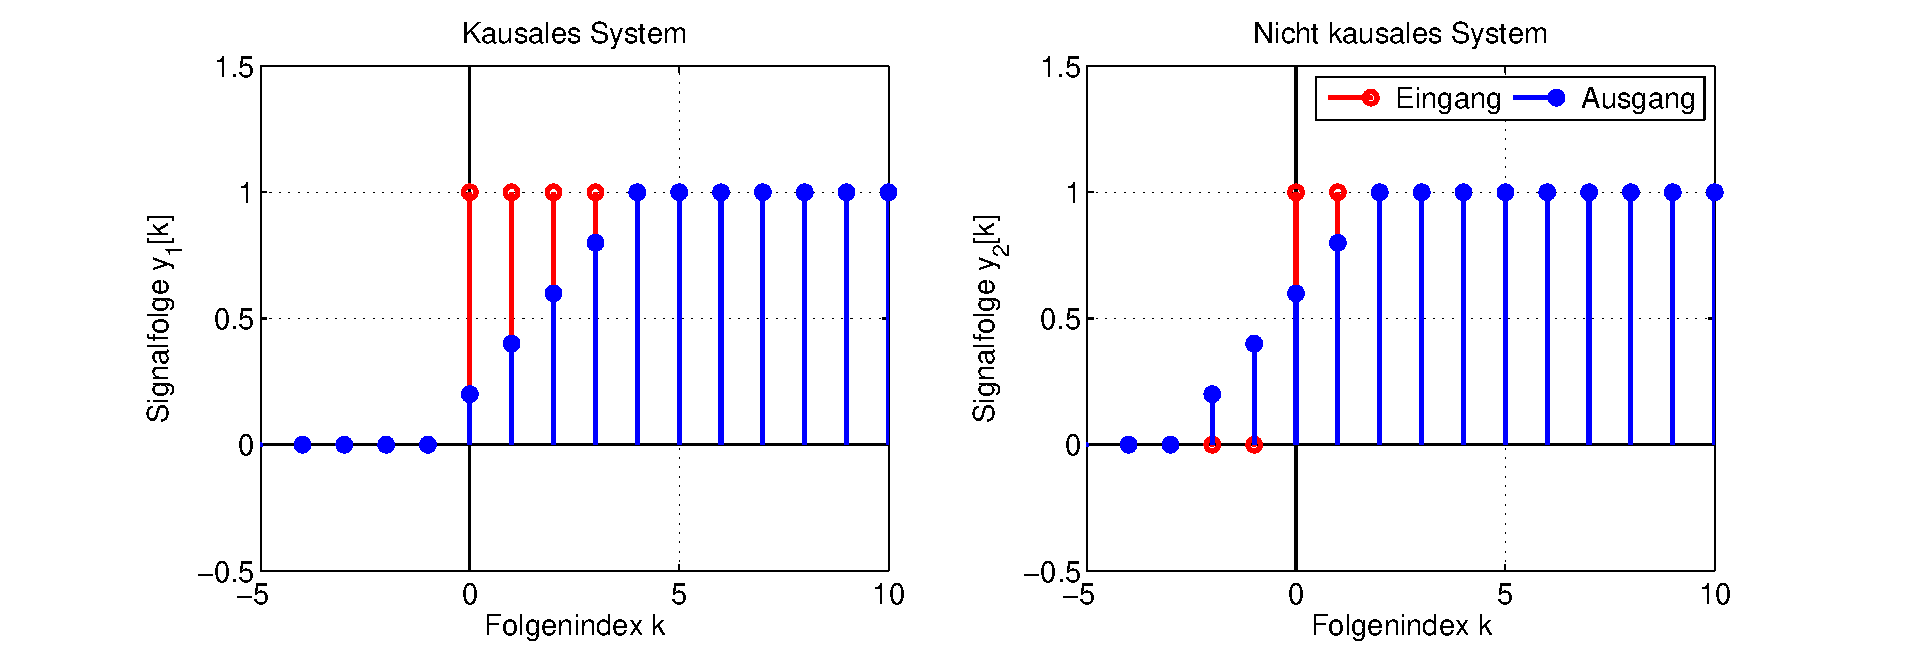
\includegraphics[width=1\textwidth]{Kapitel4/Bilder/image9.eps}}
  \caption{Sprungantwort eines kausalen und eines nicht kausalen Systems zur Berechnung eines gleitenden Mittelwertes}
  \label{fig:GleitenderMittelwertKausal}
\end{figure}

\noindent Es ist deutlich zu erkennen, dass das nicht kausale System reagiert, bevor der Sprung des Eingangssignals stattgefunden hat, w\"{a}hrend das kausale Signal erst nach der eigentlichen Anregung reagiert.

\subsubsection{Stabilit\"{a}t}

\noindent F\"{u}r zeitkontinuierliche Systeme wird in Teil A der Buchreihe folgende Stabilit\"{a}tsdefinition eingef\"{u}hrt: Ein System ist asymptotisch stabil, wenn es nach einer zeitlich begrenzten Anregung mit endlicher Energie wieder seine Ruheposition erreicht. Es ist grenzstabil, wenn es nach einer zeitlich begrenzten Anregung mit endlicher Energie zu einem konstanten Ausgangswert konvergiert oder mit konstant schwingendem Ausgangssignal reagiert. Ein System ist instabil, wenn es auf eine einer zeitlich begrenzten Anregung endlicher Energie mit divergierendem Ausgangssignal reagiert. Diese Stabilit\"{a}tsdefinition wird f\"{u}r zeitdiskrete Systeme \"{u}bernommen.\medskip

\noindent Wie bei zeitkontinuierlichen Systemen erfolgt der Nachweis im Zeitbereich \"{u}ber die charakteristische Gleichung (Kapitel 4.3.3) oder die Impulsantwort (Kapitel 4.4.4). Alternativ kann die Stabilit\"{a}t mit der z-Transformation bewertet werden (Kapitel 6.3).\bigskip

{\fontfamily{phv}\selectfont
\noindent\textbf{Stabiles, grenzstabiles und instabiles System}} \smallskip

\noindent Als Beispiele werden rekursive Systeme untersucht. Das erste System hat die Differenzengleichung 

\begin{equation}\label{eq:fourfourtyone}
y_{1} \left[k\right]=10\cdot u\left[k\right]+\frac{1}{2} \cdot y_{1} \left[k-1\right]
\end{equation}

\noindent Wird die Anregung u[k] nach einer endlichen Zeit zu null, wird der Wert y${}_{1}$[k] nur halb so gro{\ss} wie der Wert y${}_{1}$[k -- 1] im Takt zuvor. Aus diesem Grund konvergiert y${}_{1}$[k] f\"{u}r k $\rightarrow$ $\infty$ gegen null. Das System ist asymptotisch stabil. Das zweite System wird \"{u}ber die Differenzengleichung

\begin{equation}\label{eq:fourfourtytwo}
y_{2} \left[k\right]=2\cdot u\left[k\right]+y_{2} \left[k-1\right]
\end{equation}

\noindent beschrieben. Wird die Anregung u[k] zu null, bleibt der Wert y${}_{2}$[k] genauso so gro{\ss} wie der Wert y[k -- 1] im Takt zuvor. Aus diesem Grund ist y${}_{2}$[k] f\"{u}r k $\rightarrow$ $\infty$ konstant. Das System ist grenzstabil. Das dritte System wird durch die Gleichung 

\begin{equation}\label{eq:fourfourtythree}
y_{3} \left[k\right]=\frac{1}{2} \cdot u\left[k\right]+\frac{11}{10} \cdot y_{3} \left[k-1\right]
\end{equation}

\noindent definiert. Bereits an der Differenzengleichung wird deutlich, dass auch nach Ende der Anregung der Wert y[k] einen Faktor 1.1 gr\"{o}{\ss}er ist als der Werte y[k - 1] im Takt zuvor. Die Systemantwort divergiert. Das System ist damit instabil. Bild \ref{fig:RekursivTiefpassStabilitaet} zeigt die Sprungantworten der unterschiedlichen Systeme. Alle Systeme werden mit einer Rechteckfolge 

\begin{equation}\label{eq:fourfourtyfour}
u\left[k\right]=\sigma \left[k\right]-\sigma \left[k-10\right]
\end{equation}

\noindent angeregt, die eine endliche Energie aufweist.

\begin{figure}[H]
  \centerline{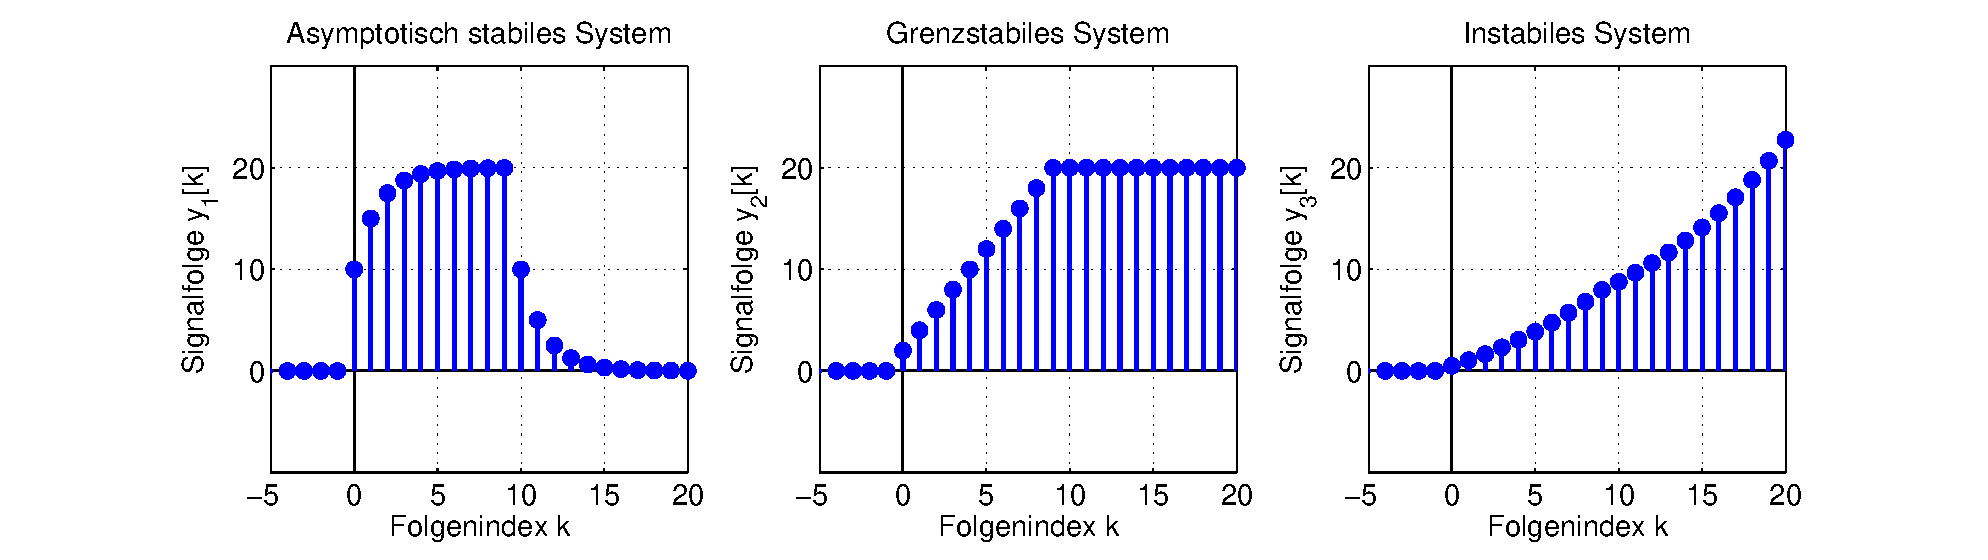
\includegraphics[width=1\textwidth]{Kapitel4/Bilder/image10.eps}}
  \caption{Sprungantwort eines asymptotisch stabilen, grenzstabilen und instabilen Systems}
  \label{fig:RekursivTiefpassStabilitaet}
\end{figure}

\noindent Bei dem asymptotisch stabilen System klingt die Systemantwort ab, wenn das Eingangssignal zu null wird. Bei dem grenzstabilen System bleibt die Systemantwort konstant, wenn die Anregung zu null wird. Bei dem instabilen System w\"{a}chst das Ausgangssignal stetig an, auch nachdem die Anregung zu null wird.\medskip

\noindent Die Stabilit\"{a}tseigenschaften lassen sich bei diesen einfachen Systemen bereits an der Differenzengleichung abgelesen, indem das Eingangssignal zu null gesetzt wird. Bei dem stabilen System ergibt sich der neue Ausgangswert aus einem Bruchteil des alten Ausgangswertes. Bei dem grenzstabilen System sind alter und neuer Ausgangswert identisch. Bei dem instabilen System ergibt sich der neue Ausgangswert aus einem Vielfachen des alten Ausgangswertes. Der Koeffizient vor dem Term y[k - 1] entscheidet bei diesem System erster Ordnung offenbar \"{u}ber die Stabilit\"{a}t des Systems.

\clearpage

\subsubsection{Zusammenfassung grundlegender Systemeigenschaften}

\noindent Tabelle \ref{tab:fourone} fasst die diskutierten Systemeigenschaften und ihre Bedeutung zusammen.

\begin{table}[H]
\setlength{\arrayrulewidth}{.1em}
\caption{Zusammenfassung von Systemeigenschaften }
\setlength{\fboxsep}{0pt}%
\colorbox{lightgray}{%
\arrayrulecolor{white}%
\begin{tabular}{| c | c |}
\hline
\parbox[c][0.35in][c]{3.3in}{\smallskip\centering\textbf{\fontfamily{phv}\selectfont{Eigenschaft}}} & \parbox[c][0.35in][c]{3.3in}{\smallskip\centering\textbf{\fontfamily{phv}\selectfont{Bedeutung}}}\\ \hline

\parbox[c][1.5in][c]{3.3in}{\centering{\fontfamily{phv}\selectfont{Linearität}}} & 
\parbox[c][1.5in][c]{3.3in}{\centering{\fontfamily{phv}\selectfont{System reagiert auf Linearkombination von Eingangssignalen \\ 
$x\left[k\right]=\nu _{1} \cdot u_{1} \left[k\right]+\nu _{2} \cdot u_{2} \left[k\right]$\\ 
mit derselben Linearkombination von Ausgangssignalen \\ 
$y\left[k\right]=\nu _{1} \cdot y_{1} \left[k\right]+\nu _{2} \cdot y_{2} \left[k\right]$}}}\\ \hline 

\parbox[c][0.64in][c]{3.3in}{\centering{\fontfamily{phv}\selectfont{Zeitinvarianz}}} & 
\parbox[c][0.64in][c]{3.3in}{\centering{\fontfamily{phv}\selectfont{System reagiert auf ein verz\"{o}gertes Eingangssignal $u[k - k{}_{0}]$ mit einem Ausgangsignal $y[k - k{}_{0}]$}}}\\ \hline


\parbox[c][0.64in][c]{3.3in}{\centering{\fontfamily{phv}\selectfont{Kausalität}}} & \parbox[c][0.64in][c]{3.3in}{\centering{\fontfamily{phv}\selectfont{System reagiert auf ein Eingangssignal erst nach Beginn der Anregung $c_{0} \neq 0$}}}\\ \hline

\parbox[c][0.64in][c]{3.3in}{\centering{\fontfamily{phv}\selectfont{Asymptotische Stabilität}}} & 
\parbox[c][0.64in][c]{3.3in}{\centering{\fontfamily{phv}\selectfont{System erreicht nach einer Anregung mit endlicher Energie wieder seine Ruheposition}}}\\ \hline

\parbox[c][0.64in][c]{3.3in}{\centering{\fontfamily{phv}\selectfont{Grenzstabilität}}} & 
\parbox[c][0.64in][c]{3.3in}{\centering{\fontfamily{phv}\selectfont{System bleibt nach einer Anregung in der aktuellen Position}}}\\ \hline

\parbox[c][0.64in][c]{3.3in}{\centering{\fontfamily{phv}\selectfont{Instabilität}}} & 
\parbox[c][0.64in][c]{3.3in}{\centering{\fontfamily{phv}\selectfont{System reagiert nach einer Anregung mit endlicher Energie mit einer divergierenden Systemantwort}}}\\ \hline

\end{tabular}%
}
\label{tab:fourone}
\end{table}

\clearpage

\subsection{L\"{o}sung linearer Differenzengleichungen mit konstanten Koeffizienten}\label{fourthree}

\noindent Die dargestellten Beispiele haben ein Systemverhalten, das \"{u}ber lineare Differenzengleichungen N-ter Ordnung mit konstanten Koeffizienten beschrieben wird. Zur Berechnung des Ausgangssignals im Zeitbereich stehen unterschiedliche Methoden zur Verf\"{u}gung, die in diesem Kapitel vorgestellt werden.

\subsubsection{Rekursive Darstellung von Differenzengleichungen}

\noindent Die Differenzengleichung N-ter Ordnung mit konstanten Koeffizienten lautet in ihrer allgemeinen Form

\begin{equation}\label{eq:fourfourtyfive}
\sum _{n=0}^{N}c_{n} \cdot y\left[k-n\right] =\sum _{l=0}^{L}d_{l} \cdot u\left[k-l\right] 
\end{equation}

\noindent Ohne Beschr\"{a}nkung der Allgemeinheit wird die Annahme c${}_{0}$ = 1 getroffen. Mit dieser Annahme kann die Gleichung umgeformt werden zu

\begin{equation}\label{eq:fourfourtysix}
y\left[k\right]=\sum _{l=0}^{L}d_{l} \cdot u\left[k-l\right] -\sum _{n=1}^{N}c_{n} \cdot y\left[k-n\right] 
\end{equation}

\noindent Das aktuelle Ausgangssignal ergibt sich allgemein aus dem aktuellen Wert des Eingangssignals sowie den vergangenen Werten des Ein- und Ausgangssignals. Die Ausgangssignale der oben dargestellten Systeme werden mit Hilfe dieser rekursiven Darstellung berechnet.\medskip

\noindent F\"{u}r numerische Berechnungen reicht dieses L\"{o}sungsverfahren f\"{u}r lineare Differenzengleichungen mit konstanten Koeffizienten vollst\"{a}ndig aus. Die rekursive Form hat aber den Nachteil, dass keine geschlossene Form des Ausgangssignals angegeben werden kann. Sie ist deshalb nicht geeignet f\"{u}r eine Analyse von Eigenschaften wie Schwingungsneigung und Stabilit\"{a}t. Deshalb werden in diesem Abschnitt Verfahren zur analytischen Berechnung der Systemantwort beschrieben.

\subsubsection{Explizite L\"{o}sung \"{u}ber die Vier-Schritt-Methode}\label{fourthreetwo}

\noindent F\"{u}r die Diskussion von Systemeigenschaften ist es notwendig, eine geschlossene Darstellung des Ausgangssignals zu erhalten. F\"{u}r die L\"{o}sung von linearen Differenzengleichungen mit konstanten Koeffizienten gibt es eine sogenannte Vier-Schritt-Methode. Sie besteht aus den Schritten

\begin{itemize}
\item  Berechnung der allgemeinen homogenen L\"{o}sung
\item  Berechnung einer partikul\"{a}ren L\"{o}sung
\item  Kombination von homogener und partikul\"{a}rer L\"{o}sung
\item  Bestimmung der Konstanten \"{u}ber Anfangsbedingungen
\end{itemize}

\clearpage


{\fontfamily{phv}\selectfont
\noindent\textbf{Berechnung der allgemeinen homogenen Lösung}} \smallskip

\noindent Zur Berechnung der allgemeinen homogenen L\"{o}sung wird das Eingangssignal auf null gesetzt. Es ergibt sich die homogene Differenzengleichung

\begin{equation}\label{eq:fourfourtyseven}
y_{H} \left[k\right]+\sum _{n=1}^{N}c_{n} \cdot y_{H} \left[k-n\right] =0
\end{equation}

\noindent Mit dem Ansatz

\begin{equation}\label{eq:fourfourtyeight}
y_{H} \left[k\right]=Y_{0} \cdot \lambda ^{k} 
\end{equation}

\noindent kann die homogene L\"{o}sung gefunden werden. Einsetzen des Ansatzes f\"{u}hrt zu der Gleichung

\begin{equation}\label{eq:fourfourtynine}
Y_{0} \cdot \lambda ^{k} +Y_{0} \cdot \sum _{n=1}^{N}c_{n} \cdot Y_{0} \cdot \lambda ^{k-n}  =0
\end{equation}

\noindent beziehungsweise

\begin{equation}\label{eq:fourfifty}
\lambda ^{k} +\sum _{n=1}^{N}c_{n} \cdot \lambda ^{k-n}  =0
\end{equation}

\noindent Sie wird als charakteristische Gleichung bezeichnet, weil mit ihr die f\"{u}r das System charakteristischen Parameter $\lambda_{n}$ bestimmt werden. Da es sich bei dem System um ein lineares System handelt, ergibt sich die allgemeine homogene L\"{o}sung aus der Linearkombination der berechneten Nullstellen $\lambda_{n}$.

\begin{equation}\label{eq:fourfiftyone}
y_{H} \left[k\right]=Y_{1} \cdot \lambda _{1}^{k} +Y_{2} \cdot \lambda _{2}^{k} +...+Y_{N} \cdot \lambda _{N}^{k}
\end{equation}

\noindent Die L\"{o}sungen der charakteristischen Gleichung m\"{u}ssen jedoch nicht die Vielfachheit von eins haben. Existiert ein N${}_{1}$-facher Wert $\lambda_{1}$, ergibt sich die allgemeine homogene L\"{o}sung

\begin{equation}\label{eq:fourfiftytwo}
y_{H} \left[k\right]=Y_{1} \cdot \lambda _{1}^{k} +Y_{2} \cdot k\cdot \lambda _{1}^{k} +...+Y_{N_{1} } \cdot k^{N_{1} -1} \cdot \lambda _{1}^{k} +Y_{N_{1} +1} \cdot \lambda _{2}^{k} +...+Y_{N} \cdot \lambda _{N-N_{1} +1}^{k}
\end{equation}

\noindent
\colorbox{lightgray}{%
\arrayrulecolor{white}%
\renewcommand\arraystretch{0.6}%
\begin{tabular}{ wl{16.5cm} }
{\fontfamily{phv}\selectfont{Beispiel: Sprungantwort eines Tiefpasses - Berechnung der allgemeinen homogenen L\"{o}sung}}
\end{tabular}%
}\medskip

\noindent Das praktische Vorgehen wird am Beispiel des rekursiven Tiefpasses dargestellt. Es soll die Systemreaktion auf einen Sprung am Eingang des Filters berechnet werden. Die Differenzengleichung f\"{u}r den Filter lautet nach Gleichung \eqref{eq:fourone}

\begin{equation}\label{eq:fourfiftythree}
y\left[k\right]=\left(1-GF\right)\cdot u\left[k\right]+GF\cdot y\left[k-1\right]
\end{equation}

\noindent F\"{u}r die allgemeine homogene L\"{o}sung muss das Eingangssignal u[k] zu null gesetzt werden.

\begin{equation}\label{eq:fourfiftyfour}
y_{H} \left[k\right]-GF\cdot y_{H} \left[k-1\right]=0
\end{equation}

\noindent Mit dem Ansatz

\begin{equation}\label{eq:fourfiftyfive}
y_{H} \left[k\right]=Y_{0} \cdot \lambda ^{k}
\end{equation}

\noindent ergibt sich

\begin{equation}\label{eq:fourfiftysix}
\lambda ^{k} -GF\cdot \lambda ^{k-1} =0
\end{equation}

\noindent Die Gleichung ist zum einen f\"{u}r $\lambda$ = 0 erf\"{u}llt. Diese triviale L\"{o}sung beschreibt aber das Ausgangssignal, das zu allen Zeiten null ist. Es ist deshalb nicht von Interesse. Die von null verschiedene Nullstelle dieser Gleichung ergibt sich zu

\begin{equation}\label{eq:fourfiftyseven}
\lambda =GF
\end{equation}

\noindent Die allgemeine homogene L\"{o}sung ergibt sich als Linearkombination der berechneten L\"{o}sungen und lautet 

\begin{equation}\label{eq:fourfiftyeight}
y_{H} \left[k\right]=Y_{0} \cdot GF^{k}
\end{equation}

\noindent Die Konstante Y${}_{0}$ wird in Schritt 4 durch Anfangsbedingungen festgelegt.\bigskip

{\fontfamily{phv}\selectfont
\noindent\textbf{Berechnung einer partikulären Lösung}} \smallskip

\noindent Im n\"{a}chsten Schritt muss eine partikul\"{a}re L\"{o}sung der Differenzengleichung

\begin{equation}\label{eq:fourfiftynine}
y_{P} \left[k\right]+\sum _{n=1}^{N}c_{n} \cdot y_{P} \left[k-n\right] =\sum _{l=0}^{L}d_{l} \cdot u\left[k-l\right]
\end{equation}

\noindent bestimmt werden. Als Ansatz f\"{u}r y${}_{P}$[k] wird ein Signal verwendet, das in Abh\"{a}ngigkeit vom Eingangssignal gew\"{a}hlt wird.


\begin{table}[H]
\setlength{\arrayrulewidth}{.1em}
\caption{Ansatz f\"{u}r partikul\"{a}re L\"{o}sungen linearer Differenzengleichungen}
\setlength{\fboxsep}{0pt}%
\colorbox{lightgray}{%
\arrayrulecolor{white}%
\begin{tabular}{| c | c |}
\hline
\parbox[c][0.35in][c]{3.3in}{\smallskip\centering\textbf{\fontfamily{phv}\selectfont{Eingangssignal $u[k]$}}} & \parbox[c][0.35in][c]{3.3in}{\smallskip\centering\textbf{\fontfamily{phv}\selectfont{Ansatz für die partikuläre Lösung $y_{P}[k]$}}}\\ \hline

\parbox[c][0.4in][c]{3.3in}{\centering{\fontfamily{phv}\selectfont{Konstante}}} & 
\parbox[c][0.4in][c]{3.3in}{\centering{\fontfamily{phv}\selectfont{Konstante}}}\\ \hline

\parbox[c][0.4in][c]{3.3in}{\centering{\fontfamily{phv}\selectfont{Polynom}}} & \parbox[c][0.4in][c]{3.3in}{\centering{\fontfamily{phv}\selectfont{Polynom gleichen Grades}}}\\ \hline

\parbox[c][0.4in][c]{3.3in}{\centering{\fontfamily{phv}\selectfont{Exponentialfolge $u_{0}^{k}$ }}} & 
\parbox[c][0.4in][c]{3.3in}{\centering{\fontfamily{phv}\selectfont{Exponentialfolge $k\cdot u_{0}^{k}$}}}\\ \hline

\parbox[c][0.4in][c]{3.3in}{\centering{\fontfamily{phv}\selectfont{Harmonische Schwingung $cos(\Omega\cdot k)$}}} & 
\parbox[c][0.4in][c]{3.3in}{\centering{\fontfamily{phv}\selectfont{$A\cdot cos(\Omega\cdot k + \varphi)$}}}\\ \hline

\end{tabular}%
}
\label{tab:fourtwo}
\end{table}

\noindent Durch Einsetzen dieses Ansatzes in die Differenzengleichung ergibt sich eine partikul\"{a}re L\"{o}sung y${}_{P}$[k]. Ist das Eingangssignal u[k] eine Kombination der dargestellten Eingangssignale, muss als Ansatz f\"{u}r die partikul\"{a}re L\"{o}sung eine entsprechende Kombination von Ans\"{a}tzen gew\"{a}hlt werden. Dabei ist es ausreichend, eine beliebige partikul\"{a}re L\"{o}sung zu finden.\medskip

\noindent Alternativ kann die partikul\"{a}re L\"{o}sung durch eine Variation der Konstanten durchgef\"{u}hrt werden. Dabei werden die Konstanten Y${}_{0}$ {\dots} Y${}_{N}$ der allgemeinen homogenen L\"{o}sung als Funktion des Index k variiert. Aufl\"{o}sen nach den variierten Konstanten Y${}_{n}$(k) f\"{u}hrt zu der gesuchten partikul\"{a}ren L\"{o}sung.

\clearpage

\noindent
\colorbox{lightgray}{%
\arrayrulecolor{white}%
\renewcommand\arraystretch{0.6}%
\begin{tabular}{ wl{16.5cm} }
{\fontfamily{phv}\selectfont{Beispiel: Sprungantwort eines Tiefpasses - Berechnung einer partikul\"{a}ren L\"{o}sung}}
\end{tabular}%
}\medskip

\noindent F\"{u}r das Beispiel des rekursiven Tiefpass-Filters wird die partikul\"{a}re L\"{o}sung \"{u}ber Variation der Konstanten bestimmt. Der Ansatz f\"{u}r die partikul\"{a}re L\"{o}sung lautet

\begin{equation}\label{eq:foursixty}
y_{P} \left[k\right]=Y_{0} \left(k\right)\cdot GF^{k} 
\end{equation}

\noindent Einsetzen in die inhomogene Differentialgleichung f\"{u}hrt unter Ber\"{u}cksichtigung des Eingangssignals 

\begin{equation}\label{eq:foursixtyone}
u\left[k\right]=\sigma \left[k\right]
\end{equation}

\noindent zu

\begin{equation}\label{eq:foursixtytwo}
Y_{0} \left(k\right)\cdot GF^{k} -GF\cdot Y_{0} \left(k-1\right)\cdot GF^{k-1} =\left(1-GF\right)\cdot \sigma \left[k\right]
\end{equation}

\noindent Damit kann der Koeffizient Y${}_{0}$(k) rekursiv beschrieben werden als

\begin{equation}\label{eq:foursixtythree}
Y_{0} \left(k\right)=Y_{0} \left(k-1\right)+\frac{\left(1-GF\right)}{GF^{k} } \cdot \sigma \left[k\right]
\end{equation}

\noindent Da nur eine beliebige partikul\"{a}re L\"{o}sung erforderlich ist, kann Y${}_{0}$(- 1) = 0 gesetzt werden. Damit sind auch alle Konstanten Y${}_{0}$(k) mit k $\mathrm{<}$ 1 null. F\"{u}r k $\mathrm{>}$ - 1 ergibt sich

\begin{equation}\label{eq:foursixtyfour}
Y_{0} \left(0\right)=\left(1-GF\right)
\end{equation}

\begin{equation}\label{eq:foursixtyfive}
Y_{0} \left(1\right)=\left(1-GF\right)+\frac{\left(1-GF\right)}{GF}
\end{equation}

\noindent Eine wiederholte Berechnung f\"{u}hrt auf Y${}_{0}$(k) 

\begin{equation}\label{eq:foursixtysix}
Y_{0} \left(k\right)=\left(1+\frac{1}{GF} +\left(\frac{1}{GF} \right)^{2} +...+\left(\frac{1}{GF} \right)^{k} \right)\cdot \left(1-GF\right)\cdot \sigma \left[k\right]
\end{equation}

\noindent Mit der Summenformel f\"{u}r die endliche geometrische Reihe ergibt sich wegen der Definition des Ged\"{a}chtnisfaktors mit {\textbar}GF{\textbar} $\mathrm{<}$ 1

\begin{equation}\label{eq:foursixtyseven}
Y_{0} \left(k\right)=\left(\frac{1-\left(\frac{1}{GF} \right)^{k+1} }{1-\frac{1}{GF} } \right)\cdot \left(1-GF\right)\cdot \sigma \left[k\right]
\end{equation}

\noindent und die partikul\"{a}re L\"{o}sung lautet

\begin{equation}\label{eq:foursixtyeight}
y_{P} \left[k\right]=\left(\frac{1-\left(\frac{1}{GF} \right)^{k+1} }{1-\frac{1}{GF} } \right)\cdot \left(1-GF\right)\cdot \sigma \left[k\right]\cdot GF^{k} =\left(1-GF^{k+1} \right)\cdot \sigma \left[k\right]
\end{equation}

\clearpage

{\fontfamily{phv}\selectfont
\noindent\textbf{ Kombination von allgemeiner homogener und partikul\"{a}rer L\"{o}sung}} \smallskip

\noindent Die komplette L\"{o}sung der Differenzengleichung ergibt sich als Summe aus der allgemeinen homogenen und einer partikul\"{a}ren L\"{o}sung. 

\begin{equation}\label{eq:foursixtynine}
y\left[k\right]=Y_{0} \cdot \lambda _{0}^{k} +Y_{1} \cdot \lambda _{1}^{k} +...+Y_{N} \cdot \lambda _{N}^{k} +y_{P} \left[k\right]
\end{equation}

\noindent
\colorbox{lightgray}{%
\arrayrulecolor{white}%
\renewcommand\arraystretch{0.6}%
\begin{tabular}{ wl{16.5cm} }
{\fontfamily{phv}\selectfont{Beispiel: Sprungantwort eines Tiefpasses - Kombination der beiden L\"{o}sungen}}
\end{tabular}%
}\medskip

\noindent Die Summe von allgemeiner homogener und partikul\"{a}rer L\"{o}sung errechnet sich zu

\begin{equation}\label{eq:fourseventy}
y\left[k\right]=y_{H} \left[k\right]+y_{P} \left[k\right]=Y_{0} \cdot GF^{k} +\left(1-GF^{k+1} \right)\cdot \sigma \left[k\right]
\end{equation}

{\fontfamily{phv}\selectfont
\noindent\textbf{Bestimmung der Konstanten über Anfangsbedingungen}} \smallskip

\noindent Die Werte f\"{u}r Y${}_{n}$ m\"{u}ssen durch Einsetzen von Folgenwerten ermittelt werden. F\"{u}r jede Konstante Y${}_{n}$ ist ein Folgenwert als Randbedingung notwendig. \bigskip

\noindent
\colorbox{lightgray}{%
\arrayrulecolor{white}%
\renewcommand\arraystretch{0.6}%
\begin{tabular}{ wl{16.5cm} }
{\fontfamily{phv}\selectfont{Beispiel: Sprungantwort eines Tiefpasses - Bestimmung der Konstanten}}
\end{tabular}%
}\medskip

\noindent F\"{u}r das vorliegende Beispiel wird vorgegeben, dass das Ausgangssignal f\"{u}r k $\mathrm{<}$ 0 null ist. F\"{u}r k = 0 ergibt sich das Ausgangssignal mit y[- 1] = 0 direkt \"{u}ber die Differenzengleichung zu

\begin{equation}\label{eq:fourseventyone}
y\left[0\right]=\left(1-GF\right)+GF\cdot 0=1-GF
\end{equation}

\noindent Der Wert Y${}_{0}$ in Gleichung \eqref{eq:fourseventy} muss \"{u}ber die Anfangsbedingungen y[0] = 1 - GF bestimmt werden. 

\begin{equation}\label{eq:fourseventytwo}
y\left[0\right]=Y_{0} \cdot GF^{0} +1-GF^{1} =Y_{0} +1-GF=1-GF
\end{equation}

\noindent Es ergibt sich die Konstante Y$_{0}$ = 0, und die L\"{o}sung der Differenzengleichung lautet

\begin{equation}\label{eq:fourseventythree}
y\left[k\right]=\left(1-GF^{k+1} \right)\cdot \sigma \left[k\right]
\end{equation}

\noindent Bild \ref{fig:RCRekursivAnalytisch} vergleicht das Ausgangssignal der rekursiven Berechnung mit dem der analytischen Berechnung. 

\clearpage

\begin{figure}[H]
  \centerline{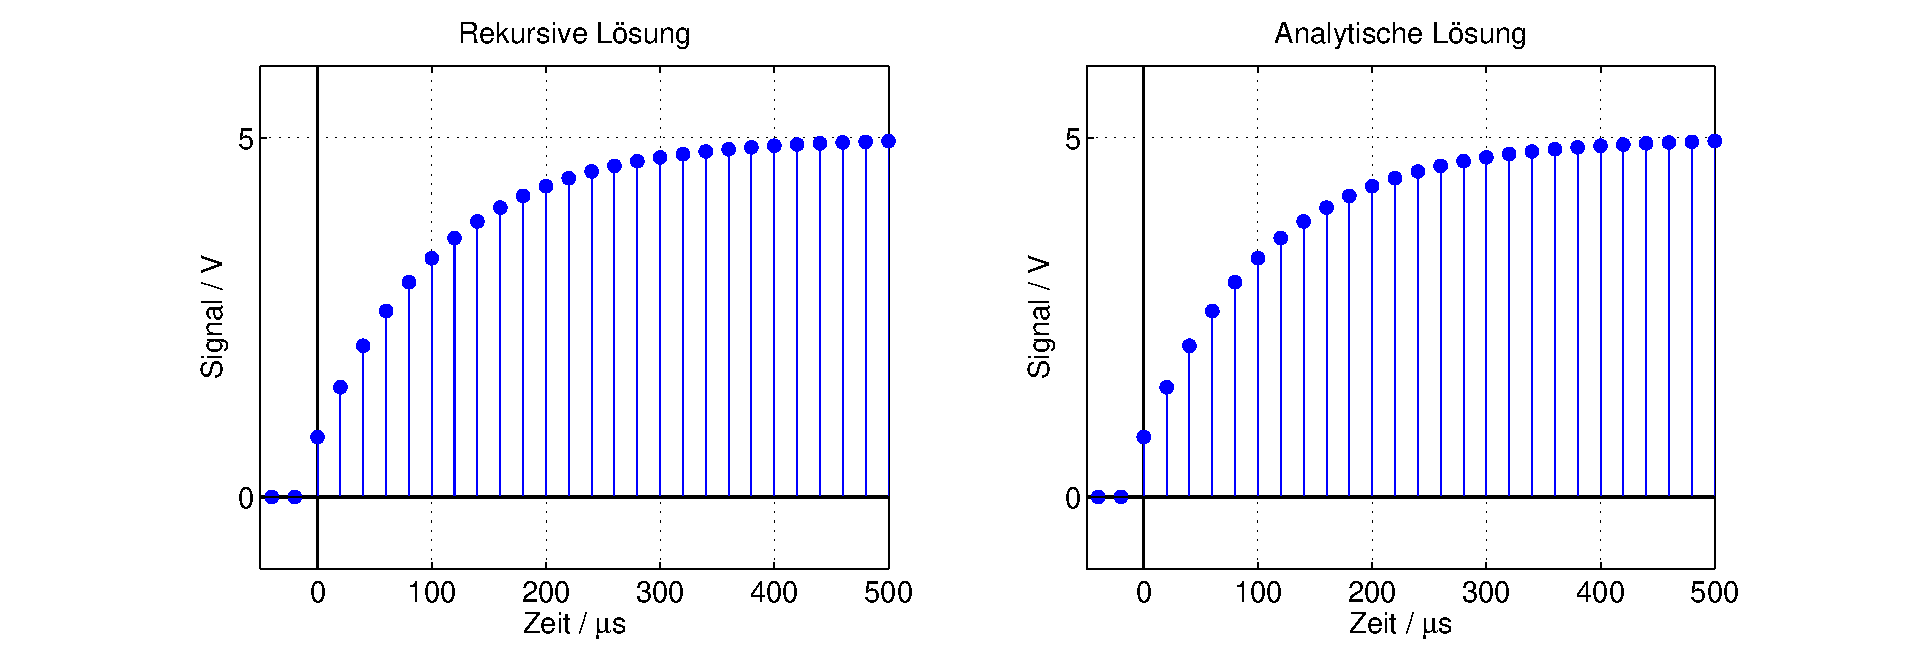
\includegraphics[width=1\textwidth]{Kapitel4/Bilder/image11.eps}}
  \caption{Vergleich zwischen rekursiver und analytischer Berechnung des Ausgangssignals eines rekursiven Tiefpass f\"{u}r GF = 0.9}
  \label{fig:RCRekursivAnalytisch}
\end{figure}

\noindent Erwartungsgem\"{a}{\ss} stimmen die beiden Berechnungen \"{u}berein.\bigskip

\noindent Das Vorgehen bei der Vier-Schritt-Methode zur L\"{o}sung linearer Differenzengleichungen mit konstanten Koeffizienten ist in Tabelle \ref{tab:fourthree} zusammengefasst.

\begin{table}[H]
\setlength{\arrayrulewidth}{.1em}
\caption{Ansatz f\"{u}r partikul\"{a}re L\"{o}sungen linearer Differenzengleichungen}
\setlength{\fboxsep}{0pt}%
\colorbox{lightgray}{%
\arrayrulecolor{white}%
\begin{tabular}{| c | c |}
\hline
\parbox[c][0.35in][c]{0.5in}{\smallskip\centering\textbf{\fontfamily{phv}\selectfont{Schritt}}} & \parbox[c][0.35in][c]{6in}{\smallskip\centering\textbf{\fontfamily{phv}\selectfont{Beschreibung}}}\\ \hline

\parbox[c][2.3in][c]{0.5in}{\centering{\fontfamily{phv}\selectfont{1}}} & 
\parbox[c][2.3in][c]{6in}{\centering{\fontfamily{phv}\selectfont{L\"{o}sung der homogenen Differenzengleichung\\ 
$\sum _{n=0}^{N}c_{n} \cdot y\left[k-n\right] =0$\\ 
\"{u}ber Ansatz\\ 
$y_{H} \left[k\right]=Y_{0} \cdot \lambda ^{k} $\\ 
durch Lösen der charakteristischen Gleichung \\
$\lambda ^{k} \sum _{n=0}^{N}c_{n}$ \\
Allgemeine Lösung in Abhängigkeit der Vielfachheit}}}\\ \hline

\parbox[c][0.4in][c]{0.5in}{\centering{\fontfamily{phv}\selectfont{2}}} & \parbox[c][0.4in][c]{6in}{\centering{\fontfamily{phv}\selectfont{Polynom gleichen Grades}}}\\ \hline

\parbox[c][0.4in][c]{0.5in}{\centering{\fontfamily{phv}\selectfont{3}}} & 
\parbox[c][0.4in][c]{6in}{\centering{\fontfamily{phv}\selectfont{Exponentialfolge $k\cdot u_{0}^{k}$}}}\\ \hline

\parbox[c][0.4in][c]{0.5in}{\centering{\fontfamily{phv}\selectfont{4}}} & 
\parbox[c][0.4in][c]{6in}{\centering{\fontfamily{phv}\selectfont{$A\cdot cos(\Omega\cdot k + \varphi)$}}}\\ \hline

\end{tabular}%
}
\label{tab:fourthree}
\end{table}

\clearpage

\subsubsection{Stabilit\"{a}t und charakteristische Gleichung eines Systems}

\noindent Bei der Einf\"{u}hrung des Begriffes der Stabilit\"{a}t in Abschnitt \ref{fourtwothree} wird ausgef\"{u}hrt, dass stabile Systeme nach einer Anregung mit endlicher Energie wieder in ihren Ausgangszustand zur\"{u}ckkehren. Das Verhalten des Systems nach der Anregung wird durch die homogene L\"{o}sung der Differentialgleichung beschrieben, die in Abschnitt \ref{fourthreetwo} berechnet wird. Sie setzt sich bei einfachen L\"{o}sungen $\lambda_{n}$ aus einer Linearkombination von Potenzfolgen zusammen. 

\begin{equation}\label{eq:fourseventyfour}
y_{H} \left[k\right]=Y_{1} \cdot \lambda _{1}^{k} +Y_{2} \cdot \lambda _{2}^{k} +...+Y_{N} \cdot \lambda _{N}^{k} 
\end{equation}

\noindent Damit die homogene L\"{o}sung zu null wird, m\"{u}ssen die alle L\"{o}sungen $\lambda$${}_{n}$ einen Betrag {\textbar}$\lambda$${}_{n}${\textbar} $\mathrm{<}$ 1 aufweisen. Besitzt ein Wert $\lambda_{n}$ einen Betrag {\textbar}$\lambda_{n}${\textbar} $\mathrm{>}$ 1, divergiert der entsprechende Summand aus Gleichung~\eqref{eq:fourseventyfour}, und folglich divergiert auch die L\"{o}sung der homogenen Differentialgleichung.\medskip

\noindent Liegt mit $\lambda_{1}$ eine P-fache L\"{o}sung der charakteristischen Gleichung vor, weisen die zugeh\"{o}rigen Summanden der homogenen L\"{o}sung Terme der Form 

\begin{equation}\label{eq:fourseventyfive}
y_{H} \left[k\right]=Y_{1} \cdot \lambda _{1}^{k} +Y_{2} \cdot k\cdot \lambda _{1}^{k} +...+Y_{P} \cdot k^{P-1} \cdot \lambda _{1}^{k} +Y_{P+1} \cdot \lambda _{2}^{k} +...+Y_{N} \cdot \lambda _{N-P+1}^{k}
\end{equation}

\noindent auf. Da die Exponentialfunktion schneller f\"{a}llt und w\"{a}chst als jede Potenz von k, konvergiert diese Summe ebenfalls f\"{u}r einen Betrag {\textbar}$\lambda_{n}${\textbar} $\mathrm{<}$ 1, und sie divergiert f\"{u}r einen Betrag {\textbar}$\lambda_{n}${\textbar} $\mathrm{>}$ 1. Dabei ist es unerheblich, ob die L\"{o}sungen $\lambda_{n}$ reell oder komplex sind.\medskip

\noindent Einen Sonderfall stellen L\"{o}sungen mit einem Betrag {\textbar}$\lambda_{n}${\textbar} = 1 dar. 

\begin{equation}\label{eq:fourseventysix}
y_{H} \left[k\right]=Y_{1} \cdot 1^{k} +Y_{2} \cdot e^{j\cdot \varphi } +Y_{3} \cdot e^{-j\cdot \varphi } +...
\end{equation}

\noindent Die L\"{o}sungen sind konstant beziehungsweise schwingen mit konstanter Amplitude. F\"{u}r den Fall einfacher L\"{o}sungen liegt damit weder eine konvergente, noch eine divergente L\"{o}sung vor. Der Fall entspricht dem diskutierten Fall der Grenzstabilit\"{a}t des zugeh\"{o}rigen Systems. \medskip

\noindent Besitzt eine L\"{o}sung mit einem Betrag {\textbar}$\lambda_{n}${\textbar} = 1 eine Vielfachheit von P $\mathrm{>}$ 1, entstehen Terme der Form

\begin{equation}\label{eq:fourseventyseven}
\begin{split}
y_{H} \left[k\right] = & \; Y_{1} \cdot 1^{k} +Y_{2} \cdot k\cdot 1^{k} +Y_{3} \cdot k^{2} \cdot 1^{k} ... \\ 
& + Y_{3} \cdot e{}^{j\cdot \varphi \cdot k} +Y{}_{4} \cdot k\cdot e{}^{j\cdot \varphi \cdot k} +Y{}_{5} \cdot k{}^{2} \cdot e{}^{j\cdot \varphi \cdot k} ... \\ 
& + Y{}_{6} \cdot e{}^{-j\cdot \varphi \cdot k} +Y{}_{7} \cdot k\cdot e{}^{-j\cdot \varphi \cdot k} +Y{}_{8} \cdot k{}^{2} \cdot e{}^{-j\cdot \varphi \cdot k} ...
\end{split}
\end{equation}

\noindent Da die Exponentialfunktion die Terme nicht d\"{a}mpft, divergiert der Ausdruck und damit die gesamte homogene L\"{o}sung. Das System ist instabil. Aus dieser Diskussion ergibt sich der in Tabelle 4.7 beschriebene Zusammenhang zwischen der Stabilit\"{a}t von linearen, zeitinvarianten Systemen und den L\"{o}sungen der charakteristischen Gleichung.

\clearpage

\begin{table}[H]
\setlength{\arrayrulewidth}{.1em}
\caption{Zusammenhang zwischen L\"{o}sungen der charakteristischen Gleichung und der Stabilit\"{a}t von LTI-Systemen}
\setlength{\fboxsep}{0pt}%
\colorbox{lightgray}{%
\arrayrulecolor{white}%
\begin{tabular}{| c | c |}
\hline
\parbox[c][0.35in][c]{3.4in}{\smallskip\centering\textbf{\fontfamily{phv}\selectfont{Eigenschaft}}} & \parbox[c][0.35in][c]{3.4in}{\smallskip\centering\textbf{\fontfamily{phv}\selectfont{L\"{o}sungen $\lambda_{n}$ der charakteristischen Gleichung}}}\\ \hline

\parbox[c][0.8in][c]{3.4in}{\centering{\fontfamily{phv}\selectfont{Asymptotisch stabiles System}}} & 
\parbox[c][0.8in][c]{3.4in}{\centering{\fontfamily{phv}\selectfont{Alle L\"{o}sungen $\lambda_{n}$ besitzen einen\\ Betrag {\textbar}$\lambda_{n}${\textbar} $\mathrm{<} 1$}}}\\ \hline

\parbox[c][1in][c]{3.4in}{\centering{\fontfamily{phv}\selectfont{Grenzstabiles System}}} & \parbox[c][1in][c]{3.4in}{\centering{\fontfamily{phv}\selectfont{Alle L\"{o}sungen $\lambda_{n}$ besitzen einen\\ Betrag {\textbar}$\lambda_{n}${\textbar} $\mathrm{<} 1$,\\ zus\"{a}tzlich liegt mindestens\\ eine einfache L\"{o}sung mit Betrag {\textbar}$\lambda_{n}${\textbar}$ = 1$ vor }}}\\ \hline

\parbox[c][1in][c]{3.4in}{\centering{\fontfamily{phv}\selectfont{Instabiles System}}} & 
\parbox[c][1in][c]{3.4in}{\centering{\fontfamily{phv}\selectfont{Es existiert mindestens eine L\"{o}sung $\lambda_{n}$\\ mit einem Betrag {\textbar}$\lambda_{n}${\textbar} $\mathrm{>} 1$\\ oder eine mehrfache L\"{o}sung mit Betrag {\textbar}$\lambda_{n}${\textbar}$ = 1$ }}}\\ \hline

\end{tabular}%
}
\label{tab:fourfour}
\end{table}

\subsubsection{Sprung- und Impulsantwort eines Systems}\label{fourthreefour}

\noindent Das Ausgangssignal eines zeitdiskreten Systems ist von dem Anfangszustand abh\"{a}ngig. Sind die Anfangsbedingungen null, ist das System energiefrei. Wie im zeitkontinuierlichen Bereich wird die Reaktion eines energiefreien Systems auf eine sprungf\"{o}rmige Erregung $\sigma$[k] als Sprungantwort h[k] bezeichnet.

\begin{figure}[H]
  \centerline{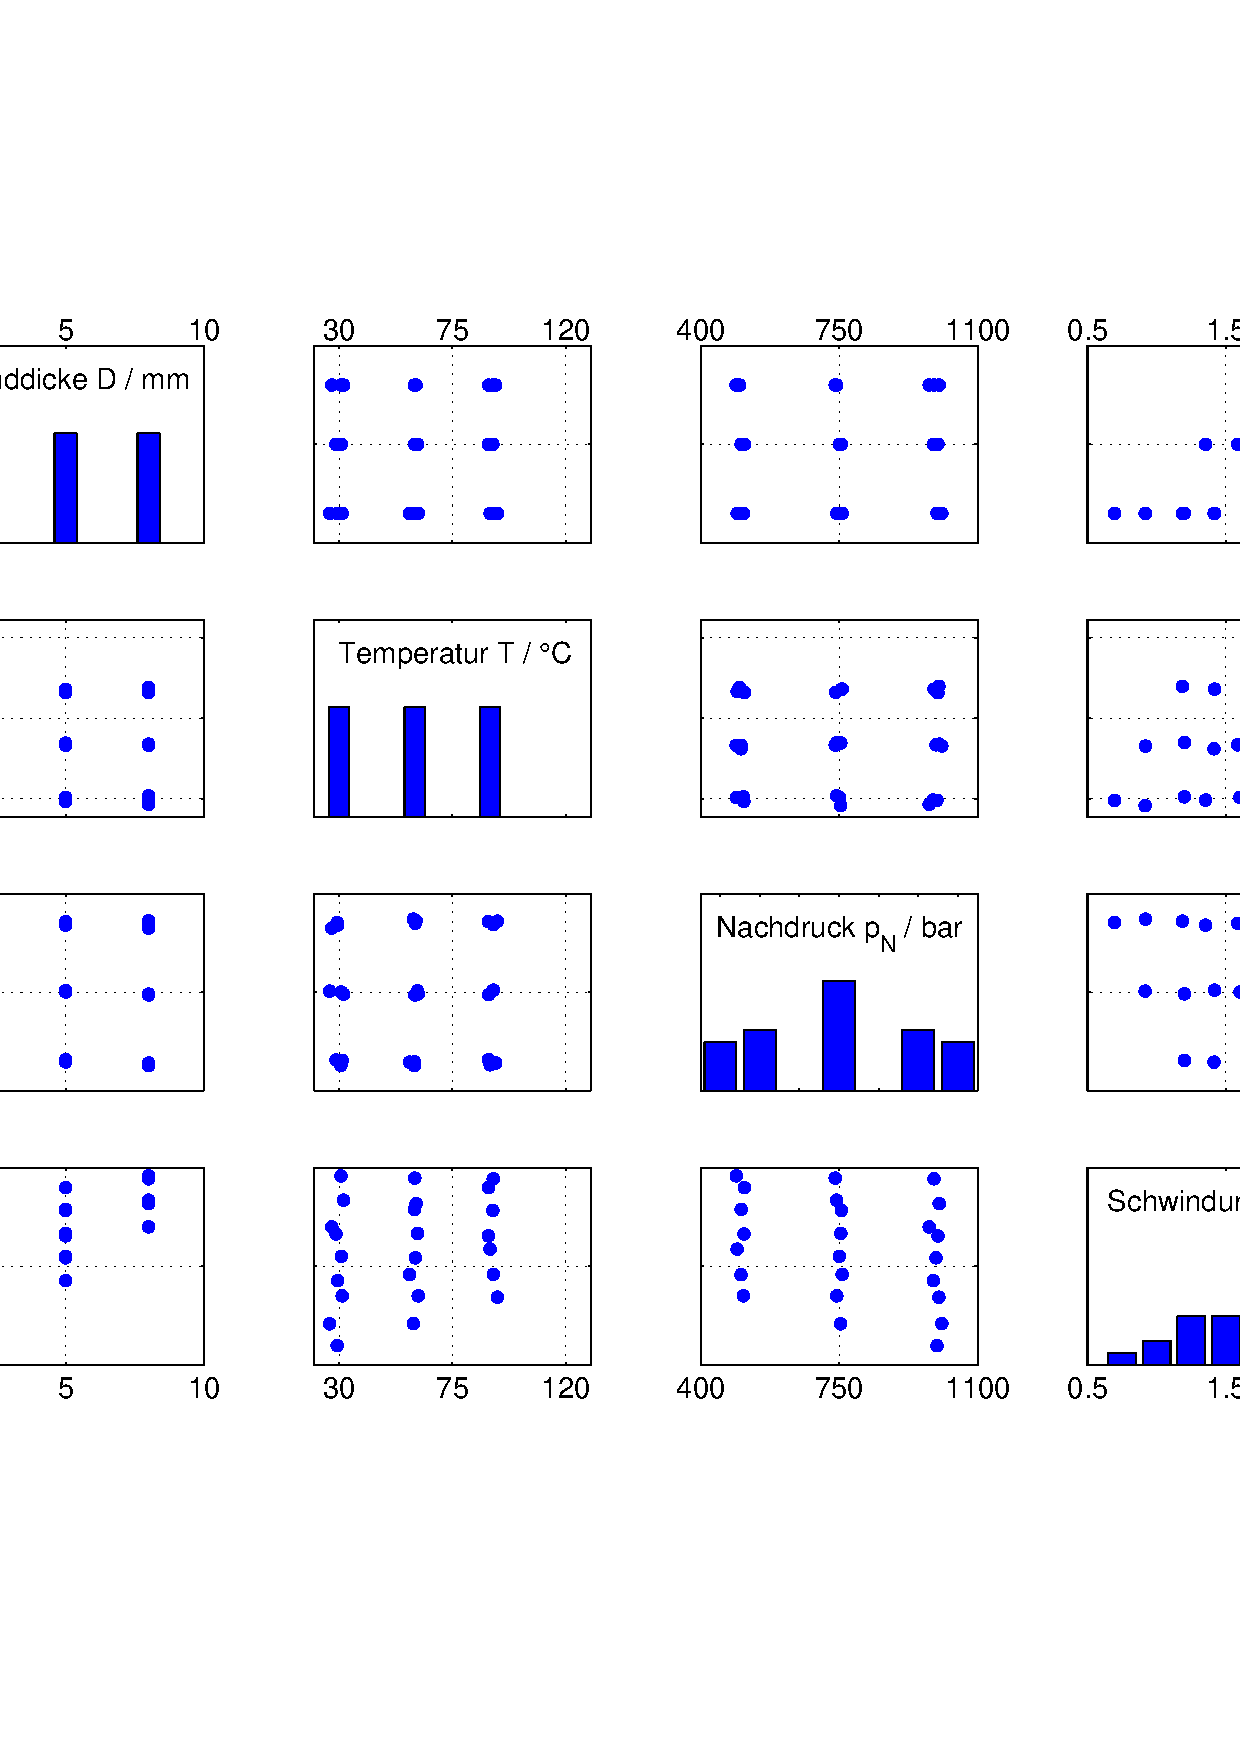
\includegraphics[width=0.6\textwidth]{Kapitel4/Bilder/image12.png}}
  \caption{Sprungantwort h[k] und Impulsantwort g[k] als Ausgangssignal eines energiefreien Systems}
  \label{fig:SystemSprungImpulsantwort}
\end{figure}

\noindent F\"{u}r das Beispiel des rekursiven Filters wird in Abschnitt 4.3.2 die Antwort des energiefreien Systems auf einen Sprung der H\"{o}he 1 mit der Bedingung y[k = - 1] = 0 berechnet.

\begin{equation}\label{eq:fourseventyeight}
y\left[k\right]=\left(1-GF^{k+1} \right)\cdot \sigma \left[k\right]
\end{equation}

\noindent Analog wird die Impulsantwort g[k] als Reaktion eines energiefreien Systems auf eine Anregung mit einem Impuls $\delta$[k] definiert. Im Kapitel \ref{threetwo} wird gezeigt, dass die Impulsfolge $\delta$[k] als Differenz zweier Sprungfolgen berechnet werden kann. 

\begin{equation}\label{eq:fourseventynine}
\delta \left[k\right]=\sigma \left[k\right]-\sigma \left[k-1\right]
\end{equation}

\noindent Wegen der Linearit\"{a}t und Zeitinvarianz errechnet sich die Systemreaktion eines energiefreien LTI-Systems auf einen Impuls am Eingang aus der Differenz zweier Sprungantworten zu

\begin{equation}\label{eq:foureighty}
g\left[k\right]=h\left[k\right]-h\left[k-1\right]
\end{equation}

\noindent Die Systemantwort g[k] eines rekursiven Filters auf einen Impuls $\delta$[k] ergibt sich demnach zu

\begin{equation}\label{eq:foureightyone}
g\left[k\right]=h\left[k\right]-h\left[k-1\right]=\left(1-GF^{k+1} \cdot \sigma \left[k\right]\right)-\left(1-GF^{k} \cdot \sigma \left[k-1\right]\right)
\end{equation}

\subsubsection{Berechnung der Systemantwort durch Superposition}

\noindent Ist ein System linear und zeitinvariant, kann ein Ausgangssignal dadurch berechnet werden, dass die Eingangssignale zerlegt, ihre jeweiligen Systemantworten berechnet und anschlie{\ss}end addiert werden. Dieses Prinzip wird als Superpositionsprinzip bezeichnet. Als erste Anwendung dieses Prinzips wird in Abschnitt \ref{fourthreefour} die Impulsantwort als Differenz zweier Sprungantworten berechnet. Wird zum Beispiel ein rekursives Filter mit der Differenzengleichung 

\begin{equation}\label{eq:foureightytwo}
y\left[k\right]=\left(1-GF\right)\cdot u\left[k\right]+GF\cdot y\left[k-1\right]
\end{equation}

\noindent mit einer Rechteckfolge der L\"{a}nge 10 und der H\"{o}he 5 beaufschlagt, kann das Eingangssignal als Summe zweier Sprungfolgen dargestellt werden

\begin{equation}\label{eq:foureightythree}
u\left[k\right]=5\cdot \left(\sigma \left[k\right]-\sigma \left[k-10\right]\right)=5\cdot \sigma \left[k\right]-5\cdot \sigma \left[k-10\right]
\end{equation}

\noindent Damit ergibt sich das Ausgangsignal y[k] aus der Summe der beiden Sprungantworten

\begin{equation}\label{eq:foureightyfour}
y\left[k\right]=5\cdot h\left[k\right]-5\cdot h\left[k-10\right]=5\cdot \left(1-GF^{k+1} \cdot \sigma \left[k\right]\right)-5\cdot \left(1-GF^{k-9} \cdot \sigma \left[k-10\right]\right)
\end{equation}

\noindent Bild \ref{fig:SuperpositionRekursiverFilter} stellt das Superpositionsprinzip f\"{u}r das Beispiel des rekursiven Filters bei Anregung mit einem rechteckf\"{o}rmigen Signal dar.

\begin{figure}[H]
  \centerline{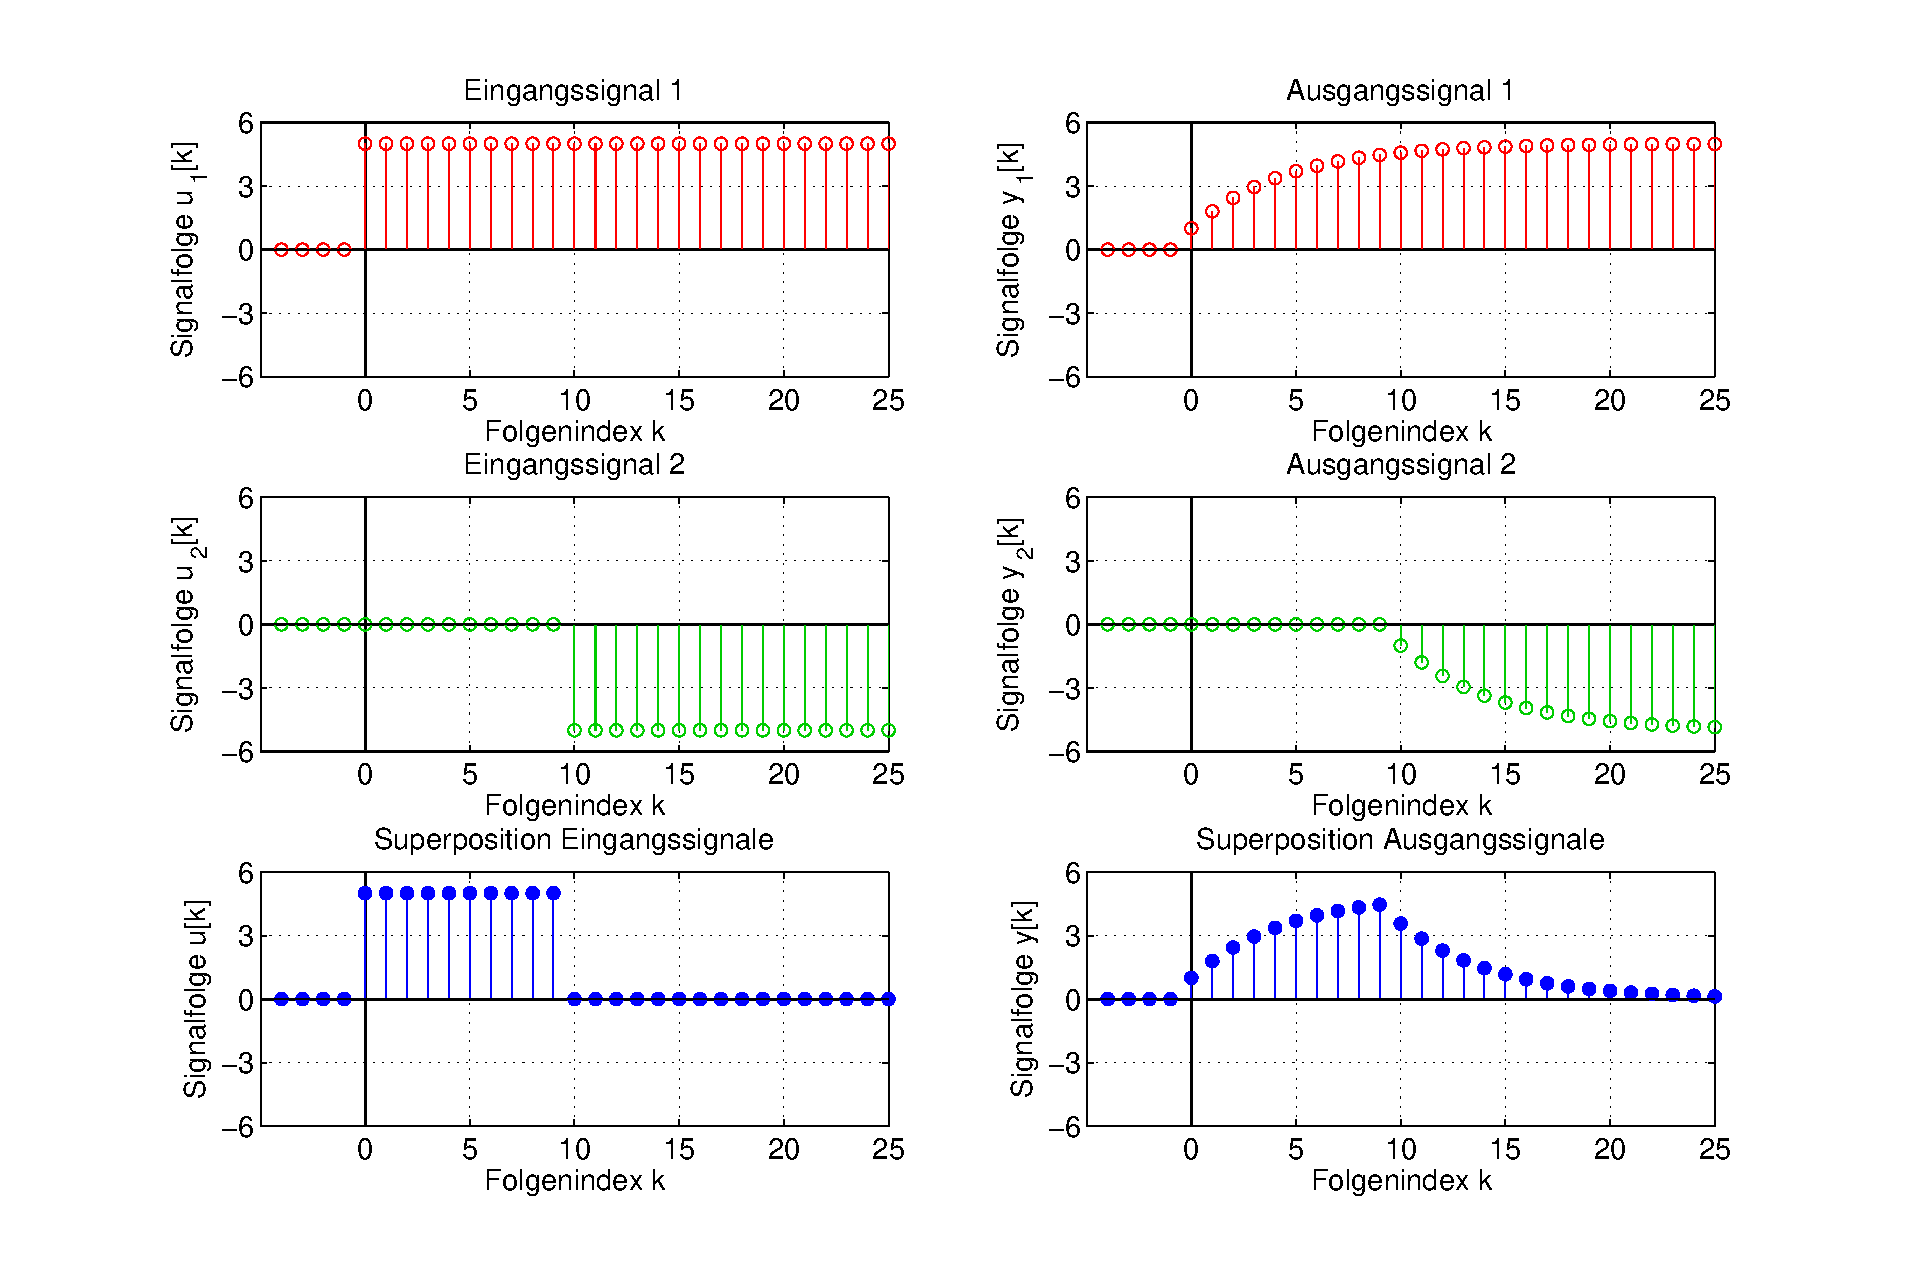
\includegraphics[width=1\textwidth]{Kapitel4/Bilder/image13.eps}}
  \caption{\"{U}berlagerung der Systemreaktion y[k] = y${}_{1}$[k]${}_{\ }$+ y${}_{2}$[k] bei \"{u}berlagertem Eingangssignal u[k] = u${}_{1}$[k]${}_{\ }$+ u${}_{2}$[k]}
  \label{fig:SuperpositionRekursiverFilter}
\end{figure}

\noindent Mit der Kenntnis der Sprungantwort eines Systems kann demnach f\"{u}r Eingangssignale, die sich \"{u}ber die Sprungfolgen darstellen lassen, eine Systemantwort \"{u}ber Superposition berechnet werden. 

\clearpage

\subsection{Berechnung der Systemantwort \"{u}ber die Faltungssumme}

\noindent Das Superpositionsprinzip erlaubt eine Zerlegung des Eingangssignals in eine Linearkombination von Eingangssignalen, deren entsprechendes Ausgangsignal bekannt ist. Auf Basis des Superpositionsprinzips kann bei bekannter Impulsantwort g[k] das Ausgangssignal zu einem beliebigen Eingangssignal u[k] bestimmt werden. Der Vorgang wird wie bei zeitkontinuierlichen Systemen als Faltung bezeichnet. Im diskreten Zeitbereich geht das Faltungsintegral in eine sogenannte Faltungssumme \"{u}ber.

\subsubsection{Herleitung der Faltungssumme}

\noindent Mathematisch kann die Faltungssumme \"{u}ber das Superpositionsprinzip hergeleitet werden. Die Systemreaktion eines energiefreien Systems auf einen Impuls am Eingang ist die Impulsantwort g[k]. Ein beliebiges Eingangssignal u[k] kann mit der Ausblendeigenschaft der Impulsfolge als gewichtete Summe von Impulsen beschrieben werden.

\begin{equation}\label{eq:foureightyfive}
u\left[k\right]=\sum _{\kappa =-\infty }^{\infty }u\left[\kappa \right]\cdot \delta \left[k-\kappa \right]
\end{equation}

\noindent Die Systemantwort y[k] auf ein solches Eingangssignal ergibt sich aus derselben Linearkombination von Impulsantworten

\begin{equation}\label{eq:foureightysix}
y\left[k\right]=\sum _{\kappa =-\infty }^{\infty }u\left[\kappa \right]\cdot g\left[k-\kappa \right] =u\left[k\right]*g\left[k\right]
\end{equation}

\noindent Diese Operation wird als Faltungssumme oder auch diskrete Faltung bezeichnet.\bigskip

\noindent
\colorbox{lightgray}{%
\arrayrulecolor{white}%
\renewcommand\arraystretch{0.6}%
\begin{tabular}{ wl{16.5cm} }
{\fontfamily{phv}\selectfont{Beispiel: Berechnung der gleitenden Mittelung \"{u}ber die Faltungssumme}}
\end{tabular}%
}\medskip

\noindent Der im vorangegangenen Abschnitt behandelte Algorithmus zur gleitenden Mittelung f\"{u}hrte zu der Differenzengleichung

\begin{equation}\label{eq:foureightyseven}
y\left[k\right]=\frac{1}{5} \cdot \left(u\left[k\right]+u\left[k-1\right]+u\left[k-2\right]+u\left[k-3\right]+u\left[k-4\right]\right)
\end{equation}

\noindent Durch Einsetzen der Impulsfolge als Eingangssignal ergibt sich die Impulsantwort zu

\begin{equation}\label{eq:foureightyeight}
g\left[k\right]=\frac{1}{5} \cdot \left(\delta \left[k\right]+\delta \left[k-1\right]+\delta \left[k-2\right]+\delta \left[k-3\right]+\delta \left[k-4\right]\right)
\end{equation}

\noindent und das Ausgangssignal zu einem beliebigen Eingangssignal kann durch die Faltungssumme berechnet werden 

\begin{equation}\label{eq:foureightynine}
\begin{split}
y\left[k\right] & = \sum _{\kappa =-\infty }^{\infty }u\left[\kappa \right]\cdot g\left[k-\kappa \right]\\
& = \sum _{\kappa =-\infty }^{\infty }u\left[\kappa \right]\cdot \frac{1}{5}\cdot  \left(\delta \left[k - \kappa \right]+\delta \left[k- \kappa-1\right]+\delta \left[k-\kappa-2\right]+\delta \left[k-\kappa-3\right]+\delta \left[k-\kappa-4\right]\right)\\
& = \frac{1}{5}\cdot \sum _{\kappa = 0 }^{4}u[k-\kappa]
\end{split}
\end{equation}

\clearpage

\subsubsection{Grafische Interpretation der Faltungssumme}

\noindent Die direkte analytische Berechnung der Faltungssumme ist nur in Ausnahmef\"{a}llen m\"{o}glich und sinnvoll, da die Zusammenfassung der Summe aufwendig ist. Im Gegensatz zur zeitkontinuierlichen Faltung kann die zeitdiskrete Faltung aber numerisch ausgef\"{u}hrt werden. Die Faltungssumme ist damit eine Realisierungsform zeitdiskreter Systeme. Zum besseren Verst\"{a}ndnis wird deshalb die Faltung an einem Beispiel zweier Folgen grafisch veranschaulicht.\bigskip

\noindent
\colorbox{lightgray}{%
\arrayrulecolor{white}%
\renewcommand\arraystretch{0.6}%
\begin{tabular}{ wl{16.5cm} }
{\fontfamily{phv}\selectfont{Beispiel: Grafische Interpretation der Faltungssumme}}
\end{tabular}%
}\medskip

\noindent Die Folge u[k] wird als Sprungfolge angenommen, die Impulsantwort g[k] ergibt sich in diesem Beispiel zu

\begin{equation}\label{eq:fourninety}
g\left[k\right]=2\cdot \sigma \left[k\right]-\sigma \left[k-2\right]-\sigma \left[k-4\right]
\end{equation}

\noindent Die Folgen sind in Bild \ref{fig:GrafischeFaltung} grafisch dargestellt.

\begin{figure}[H]
  \centerline{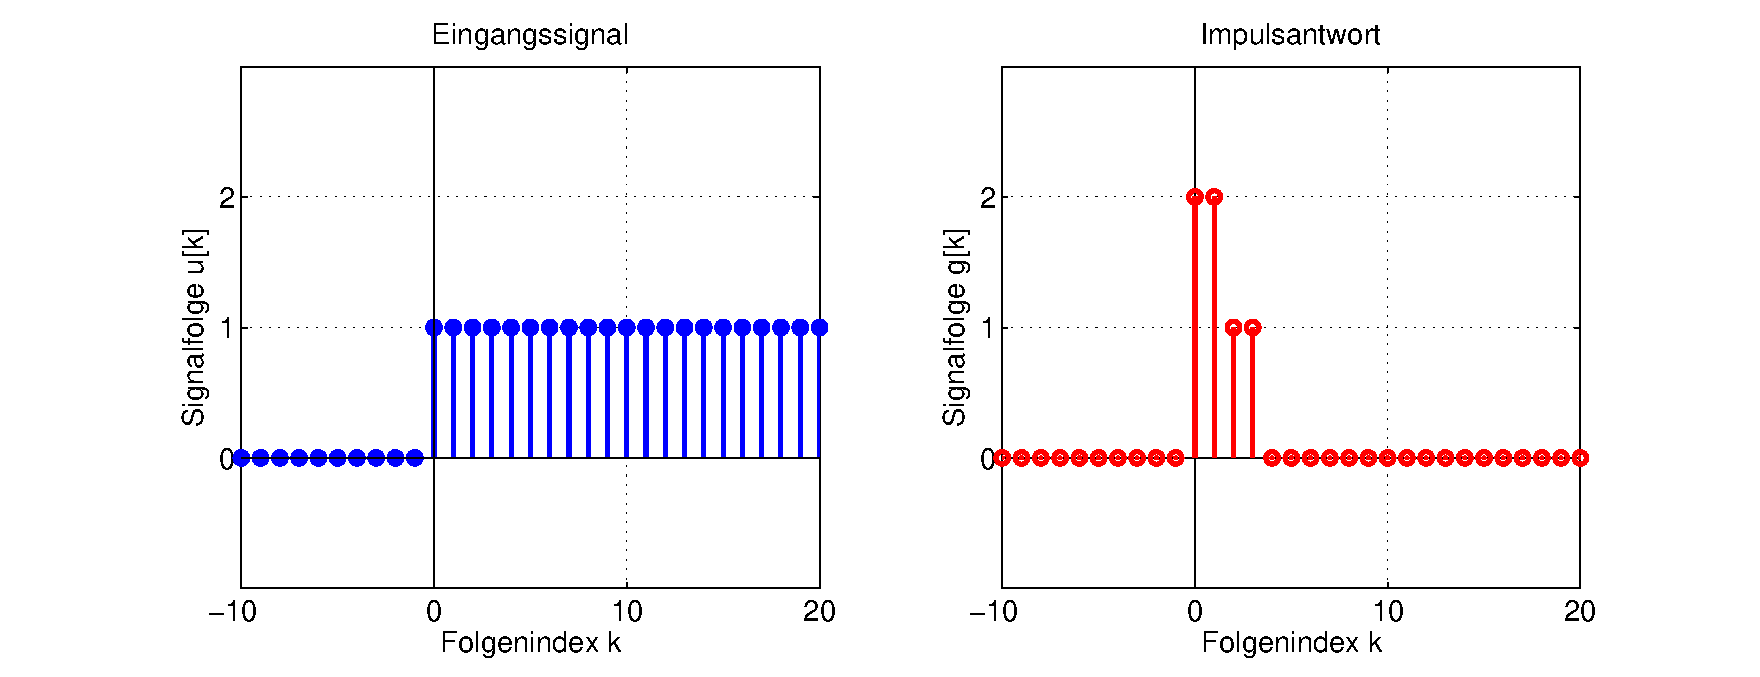
\includegraphics[width=1\textwidth]{Kapitel4/Bilder/image14.eps}}
  \caption{Folgen u[k] und g[k] f\"{u}r das Beispiel zur grafischen Interpretation der Faltungssumme}
  \label{fig:GrafischeFaltung}
\end{figure}

\noindent Die Faltung ist über eine Summenformel definiert. Sie kann umgeformt werden zu

\begin{equation}\label{eq:fourninetyone}
u\left[k\right]*g\left[k\right]=\sum _{\kappa =-\infty }^{\infty }u\left[\kappa \right]\cdot g\left[k-\kappa \right] =\sum _{\kappa =-\infty }^{\infty }u\left[\kappa \right]\cdot g\left[-(\kappa -k)\right] 
\end{equation}

\noindent Mit dieser Darstellung f\"{a}llt die Interpretation einfacher: Die Folge g[$\kappa$] wird an der Achse $\kappa = 0$ gespiegelt und um k nach rechts verschoben. Dann wird das Produkt der einzelnen Folgenwerte addiert. Bild \ref{fig:GrafischeFaltung1} stellt die unterschiedlichen Phasen der grafischen Faltung dar.

\clearpage

\begin{figure}[H]
  \centerline{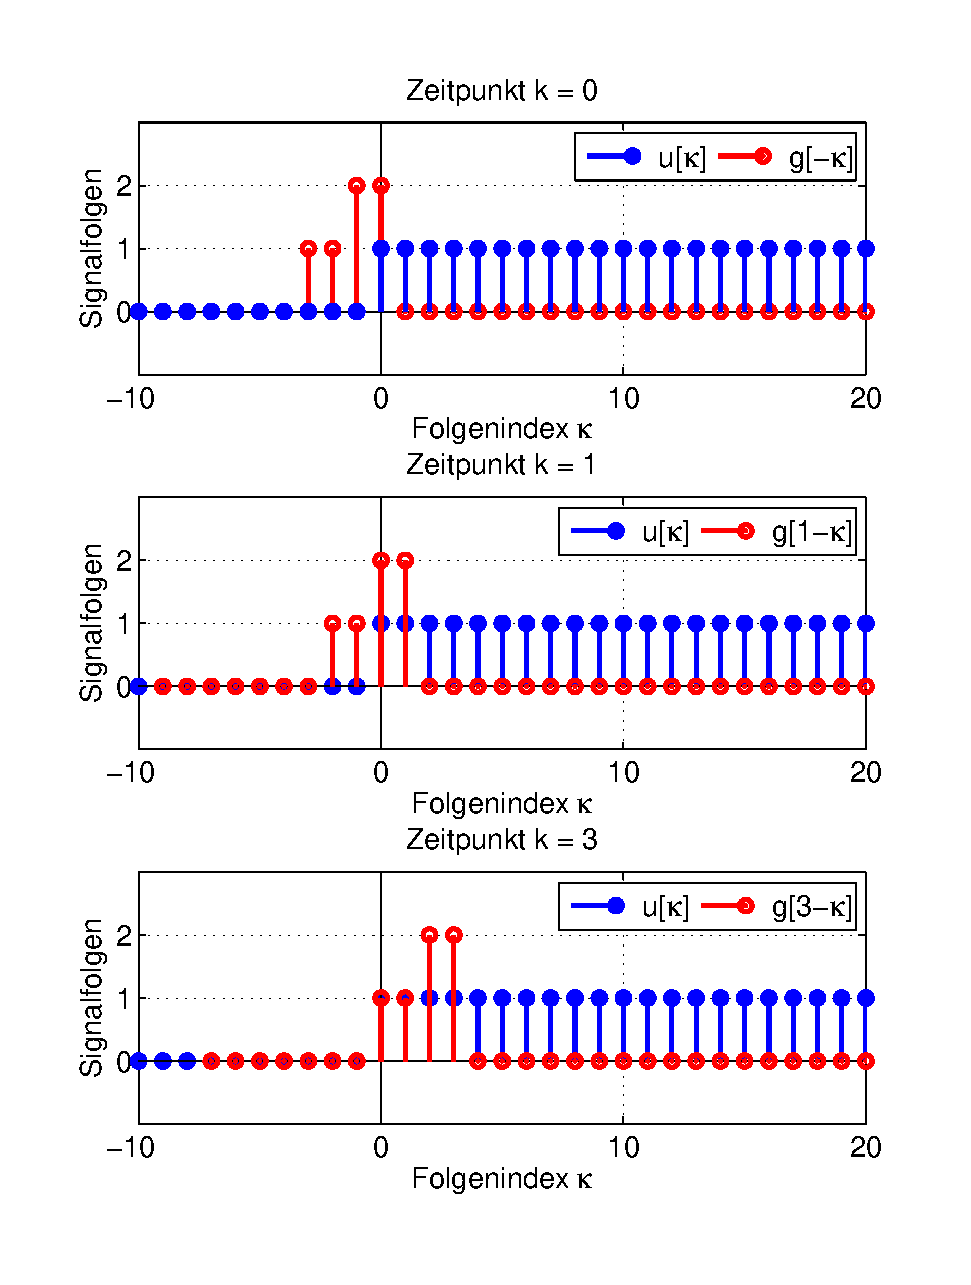
\includegraphics[width=0.5\textwidth]{Kapitel4/Bilder/image15.eps}}
  \caption{Grafische Veranschaulichung der Faltung zweier Folgen zu verschiedenen Stadien}
  \label{fig:GrafischeFaltung1}
\end{figure}

\noindent F\"{u}r negative Folgenindizes k \"{u}berschneiden sich die beiden Folgen nicht. Zum Zeitpunkt k = 0 \"{u}berschneiden sich die beiden Folgen an genau einer Stelle $\kappa$ = 0. Das Ergebnis ist damit y[0] = 2. F\"{u}r k = 1 ergibt sich eine \"{U}berschneidung der ersten beiden Werte. Nach Bildung des Produktes werden die Ergebnisse addiert und es ergibt sich y[1]= 2 + 2 = 4. So wird f\"{u}r die \"{u}brigen Werte von k fortgefahren. F\"{u}r k $\geq$ 3 \"{u}berschneidet sich die Folge x komplett mit der Folge g, sodass sich der Wert des Ausgangssignals nicht weiter \"{a}ndert. 

\begin{figure}[H]
  \centerline{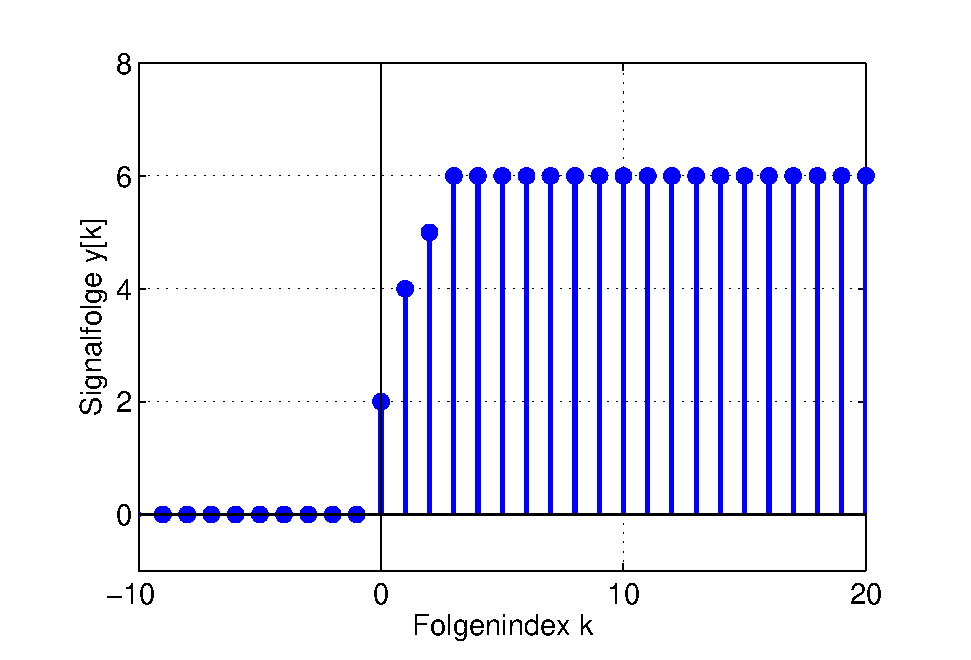
\includegraphics[width=0.5\textwidth]{Kapitel4/Bilder/image16.eps}}
  \caption{Ergebnis der Faltung zweier Folgen}
  \label{fig:GrafischeFaltung2}
\end{figure}

\noindent Aus der Grafik kann abgelesen werden, dass das Signal y[k] ab k = 3 konstant bleibt.

\clearpage

\noindent Die in diesem Beispiel dargestellte Methode zur Berechnung der Faltungssumme ist in Tabelle \ref{tab:fourfive} zusammengefasst.

\begin{table}[H]
\setlength{\arrayrulewidth}{.1em}
\caption{Vorgehen bei der Berechnung der Systemantwort über die Faltungssumme}
\setlength{\fboxsep}{0pt}%
\colorbox{lightgray}{%
\arrayrulecolor{white}%
\begin{tabular}{| c | c |}
\hline
\parbox[c][0.35in][c]{0.5in}{\smallskip\centering\textbf{\fontfamily{phv}\selectfont{Schritt}}} & \parbox[c][0.35in][c]{6in}{\smallskip\centering\textbf{\fontfamily{phv}\selectfont{Beschreibung}}}\\ \hline

\parbox[c][0.4in][c]{0.5in}{\centering{1}} & 
\parbox[c][0.4in][c]{6in}{\centering{\fontfamily{phv}\selectfont{Berechnung der Impulsantwort g[k]}}}\\ \hline

\parbox[c][0.4in][c]{0.5in}{\centering{2}} & \parbox[c][0.4in][c]{6in}{\centering{\fontfamily{phv}\selectfont{Skizze von Eingangssignal $u[k - \kappa]$ und Impulsantwort $g[k - \kappa]$}}}\\ \hline

\parbox[c][0.4in][c]{0.5in}{\centering{3}} & 
\parbox[c][0.4in][c]{6in}{\centering{\fontfamily{phv}\selectfont{Skizze von einem der Signale $u[k - \kappa]$ oder $g[k - \kappa]$ \"{u}ber Spiegelung an der Achse $\kappa = 0$ und Verschiebung um k nach rechts}}}\\ \hline

\parbox[c][0.6in][c]{0.5in}{\centering{4}} & 
\parbox[c][0.6in][c]{6in}{\centering{\fontfamily{phv}\selectfont{Aufteilen der Faltungssumme in sinnvolle Bereiche (\"{U}berlappungsbereiche, Sprungstellen, Definitionsgrenzen, ...)}}}\\ \hline

\parbox[c][0.4in][c]{0.5in}{\centering{5}} & 
\parbox[c][0.4in][c]{6in}{\centering{\fontfamily{phv}\selectfont{L\"{o}sen der Summen und Superposition der Ergebnisse}}}\\ \hline

\end{tabular}%
}
\label{tab:fourfive}
\end{table}

\InsertBoxL{0}{\includegraphics[scale=0.5]{Code.JPG}} 
\textcolor{white}{.}\newline
\noindent Im Online-Portal \textit{Systemtheorie Online} verdeutlicht die \textit{Applikation Signalabtastung und Signal-rekonstruktion} grafisch, welche Effekte durch Anti-Aliasing-Filter, reale Abtastung und reale Rekon-struktion entstehen.\newline   

\subsubsection{Rechenregeln zur Faltungssumme}

\noindent Zur Vereinfachung der Berechnung von Faltungssummen k\"{o}nnen Rechenregeln angewendet werden, die im Folgenden kurz dargestellt sind. Aus der grafischen Darstellung zur Faltung wird deutlich, dass die Faltung eine kommutative Operation ist. Der mathematische Nachweis ergibt sich aus einer Indextransformation. 

\begin{equation}\label{eq:fourninetytwo}
x_{1} \left[k\right]*x_{2} \left[k\right]=\sum _{\kappa =-\infty }^{\infty }x_{1} \left[\kappa \right]\cdot x_{2} \left[k-\kappa \right] =\sum _{k-\kappa =-\infty }^{\infty }x_{1} \left[k-\kappa \right]\cdot x_{2} \left[\kappa \right] 
\end{equation}

\noindent Da sich die Summe von - $\infty$ bis + $\infty$ erstreckt, ist eine Verschiebung um k und eine Spiegelung nicht relevant, und es ergibt sich

\begin{equation}\label{eq:fourninetythree}
x_{1} \left[k\right]*x_{2} \left[k\right]=\sum _{\kappa =-\infty }^{\infty }x_{1} \left[\kappa \right]\cdot x_{2} \left[k-\kappa \right] =\sum _{\kappa =-\infty }^{\infty }x_{1} \left[k-\kappa \right]\cdot x_{2} \left[\kappa \right] =x_{2} \left[k\right]*x_{1} \left[k\right]
\end{equation}

\noindent Das Distributivgesetz ergibt sich aus der Linearit\"{a}t der Summe.

\begin{equation}\label{eq:fourninetyfour}
\begin{split}
& \left(x_{1} \left[k\right]+x_{2} \left[k\right]\right)*x_{3} \left[k\right]=\sum _{\kappa =-\infty }^{\infty }\left(x_{1} \left[\kappa \right]+x_{2} \left[\kappa \right]\right)\cdot x_{3} \left[k-\kappa \right] \\ 
& =\sum _{\kappa =-\infty }^{\infty }x_{1} \left[\kappa \right]\cdot x_{3} \left[k-\kappa \right] +x_{2} \left[\kappa \right]\cdot x_{3} \left[k-\kappa \right]=x_{1} \left[k\right]*x_{3} \left[k\right]+x_{2} \left[k\right]*x_{3} \left[k\right]
\end{split}
\end{equation}

\noindent Das Assoziativgesetz wird hier nur genannt und nicht bewiesen. Es lautet:

\begin{equation}\label{eq:fourninetyfive}
\left(x_{1} \left[k\right]*x_{2} \left[k\right]\right)*x_{3} \left[k\right]=x_{1} \left[k\right]*\left(x_{2} \left[k\right]*x_{3} \left[k\right]\right)
\end{equation}

\noindent Bei der grafischen Faltung wird gezeigt, dass der von null verschiedene \"{U}berlappungsbereich f\"{u}r kausale Folge immer im Zahlenbereich von 0 $\dots$ k liegt. Aus diesem Grund muss die Faltung auch nur in diesem Bereich ausgef\"{u}hrt werden, sodass f\"{u}r die Faltung zweier kausaler Folgen gilt:

\begin{equation}\label{eq:fourninetysix}
\sum _{\kappa =-\infty }^{\infty }x_{1} \left[\kappa \right]\cdot x_{2} \left[k-\kappa \right] =\sum _{\kappa =0}^{k}x_{1} \left[\kappa \right]\cdot x_{2} \left[k-\kappa \right] 
\end{equation}

\noindent Aus der Eigenschaft folgt au{\ss}erdem, dass die Faltung zweier kausaler Folgen zu einer kausalen Folge f\"{u}hrt. Die Rechenregeln f\"{u}r die Faltung mit einer Impulsfolge werden in Abschnitt 3.2.1 bei der Einf\"{u}hrung von Impulsfolgen behandelt. 

\begin{table}[H]
\setlength{\arrayrulewidth}{.1em}
\caption{Zusammenfassung der Rechenregeln zur Faltungssumme}
\setlength{\fboxsep}{0pt}%
\colorbox{lightgray}{%
\arrayrulecolor{white}%
\begin{tabular}{| c | c |}
\hline
\parbox[c][0.35in][c]{3.3in}{\smallskip\centering\textbf{\fontfamily{phv}\selectfont{Rechenregel}}} & \parbox[c][0.35in][c]{3.3in}{\smallskip\centering\textbf{\fontfamily{phv}\selectfont{Darstellung als Gleichung}}}\\ \hline

\parbox[c][0.4in][c]{3.3in}{\centering{\fontfamily{phv}\selectfont{Kommutativgesetz}}} & 
\parbox[c][0.4in][c]{3.3in}{\centering{$x_{1} \left[k\right]*x_{2} \left[k\right]=x_{2} \left[k\right]*x_{1} \left[k\right]$}}\\ \hline

\parbox[c][0.4in][c]{3.3in}{\centering{\fontfamily{phv}\selectfont{Distributivgesetz}}} & \parbox[c][0.4in][c]{3.3in}{\centering{$\left(x_{1} \left[k\right]+x_{2} \left[k\right]\right)*x_{3} \left[k\right]=x_{1} \left[k\right]*x_{3} \left[k\right]+x_{2} \left[k\right]*x_{3} \left[k\right]$}}\\ \hline

\parbox[c][0.4in][c]{3.3in}{\centering{\fontfamily{phv}\selectfont{Assoziativgesetz}}} & 
\parbox[c][0.4in][c]{3.3in}{\centering{$\left(x_{1} \left[k\right]*x_{2} \left[k\right]\right)*x_{3} \left[k\right]=x_{1} \left[k\right]*\left(x_{2} \left[k\right]*x_{3} \left[k\right]\right)$}}\\ \hline

\parbox[c][0.6in][c]{3.3in}{\centering{\fontfamily{phv}\selectfont{Faltung kausaler Folgen \\
führt zu einer kausalen Folge}}} & 
\parbox[c][0.6in][c]{3.3in}{\centering{$\sum _{\kappa =-\infty }^{\infty }x_{1} \left[\kappa \right]\cdot x_{2} \left[k-\kappa \right] =\sum _{\kappa =0}^{k}x_{1} \left[\kappa \right]\cdot x_{2} \left[k-\kappa \right] $}}\\ \hline

\parbox[c][0.4in][c]{3.3in}{\centering{\fontfamily{phv}\selectfont{Faltung mit einem Impuls}}} & 
\parbox[c][0.4in][c]{3.3in}{\centering{$\delta \left[k\right]*x\left[k\right]=x\left[k\right]$}}\\ \hline

\parbox[c][0.4in][c]{3.3in}{\centering{\fontfamily{phv}\selectfont{Faltung mit einem Impuls an der Stelle $k_{0}$}}} & 
\parbox[c][0.4in][c]{3.3in}{\centering{$\delta \left[k-k_{0} \right]*x\left[k\right]=x\left[k-k_{0} \right]$}}\\ \hline

\end{tabular}%
}
\label{tab:foursix}
\end{table}

\subsubsection{Impulsantwort und Stabilit\"{a}t}

\noindent In Abschnitt 4.2.3 wird die Stabilit\"{a}t von Systemen aus physikalischer Sicht definiert. Mit dem Wissen, dass sich bei einem LTI-System die Systemantwort y[k] aus dem Faltungsintegral ergibt, kann die Stabilit\"{a}tsbewertung auf die Impulsantwort g[k] zur\"{u}ckgef\"{u}hrt werden. Dabei wird davon ausgegangen, dass das System f\"{u}r den Zeitraum 0 $\mathrm{<}$ k $\leq$ k${}_{0}$ angeregt wird. F\"{u}r den Zeitraum k $\geq$ k${}_{0\ }$nach der Anregung wird das Verhalten der Systemantwort y[k] analysiert.

\begin{equation}\label{eq:fourninetyseven}
y\left[k\right]=\sum _{\kappa =0}^{k_{0} }u\left[\kappa \right]\cdot g\left[k-\kappa \right]
\end{equation}

\noindent Aus der physikalischen Bedingung an Stabilit\"{a}t leitet sich die Forderung ab, dass bei einer zeitlich begrenzten Anregung das Ausgangssignal den Grenzwert 

\begin{equation}\label{eq:fourninetyeight}
{\mathop{\lim }\limits_{k\to \infty }} \left|y\left[k\right]\right|=0
\end{equation}

\noindent aufweisen muss. Ist der Betrag des Eingangssignals beschr\"{a}nkt, kann er mit {\textbar}u[$\kappa$]{\textbar} $\mathrm{<}$ u${}_{max}$ u${}_{MAX}$ abgesch\"{a}tzt werden, und der Betrag des Ausgangssignals kann abgesch\"{a}tzt werden mit

\begin{equation}\label{eq:fourninetynine}
\left|y\left[k\right]\right|\le \sum _{\kappa =0}^{k_{0} }\left|u\left[\kappa \right]\right|\cdot \left|g\left[k-\kappa \right]\right| \le u_{MAX} \cdot \sum _{\kappa =0}^{k_{0} }\left|g\left[k-\kappa \right]\right|
\end{equation}

\noindent Es handelt sich um eine Summe von k${}_{0}$ + 1 Folgegliedern. Die Summe wird zu null, wenn der Betrag der Impulsantwort g[k] gegen null konvergiert.

\begin{equation}\label{eq:fouronehundred}
{\mathop{\lim }\limits_{k\to \infty }} \left|g\left[k\right]\right|=0
\end{equation}

\noindent Ein System ist damit stabil, wenn die Impulsantwort gegen null konvergiert, es ist instabil, wenn die Impulsantwort divergiert. Einen Sonderfall stellen Impulsantworten g[k] dar, die f\"{u}r k $\mathrm{\to}$ $\mathrm{\infty}$ einem konstanten Wert g${}_{0}$ zustreben. Bei diesen Systemen konvergiert das Ausgangssignal f\"{u}r k $\geq$ k${}_{0}$ gegen einen konstanten Wert.

\begin{equation}\label{eq:fouronehundredone}
{\mathop{\lim }\limits_{k\to \infty }} y\left[k\right]={\mathop{\lim }\limits_{k\to \infty }} \sum _{\kappa =0}^{k_{0} }u\left[\kappa \right]\cdot g\left[k-\kappa \right] =g_{0} \cdot \sum _{\kappa =0}^{k_{0} }x\left[\kappa \right] =y_{0} 
\end{equation}

\noindent Systeme, deren Impulsantworten g[k] f\"{u}r k $\mathrm{\to}$ $\mathrm{\infty}$ einem konstanten Wert g${}_{0}$ zustreben, entsprechen damit den Bedingungen grenzstabiler Systeme. Dasselbe gilt f\"{u}r Systeme, deren Impulsantwort f\"{u}r k $\mathrm{\to}$ $\mathrm{\infty}$ mit konstanter Amplitude schwingt. Der Zusammenhang zwischen Impulsantwort und Stabilit\"{a}t linearer, zeitinvarianter Systeme ist in Tabelle \ref{tab:fourseven} zusammengefasst.

\begin{table}[H]
\setlength{\arrayrulewidth}{.1em}
\caption{Zusammenfassung des Zusammenhangs zwischen Impulsantwort und Stabilit\"{a}t von LTI-Systemen}
\setlength{\fboxsep}{0pt}%
\colorbox{lightgray}{%
\arrayrulecolor{white}%
\begin{tabular}{| c | c |}
\hline
\parbox[c][0.35in][c]{3.3in}{\smallskip\centering\textbf{\fontfamily{phv}\selectfont{Eigenschaft}}} & \parbox[c][0.35in][c]{3.3in}{\smallskip\centering\textbf{\fontfamily{phv}\selectfont{Bedeutung}}}\\ \hline

\parbox[c][0.4in][c]{3.3in}{\centering{\fontfamily{phv}\selectfont{Stabiles System}}} & 
\parbox[c][0.4in][c]{3.3in}{\centering{${\mathop{\lim }\limits_{k\to \infty }} g\left[k\right]=0$}}\\ \hline

\parbox[c][0.8in][c]{3.3in}{\centering{\fontfamily{phv}\selectfont{Grenzstabiles System}}} & 
\parbox[c][0.8in][c]{3.3in}{\centering{\fontfamily{phv}\selectfont{${\mathop{\lim }\limits_{k\to \infty }} g\left[k\right]=g_{0} $\\ oder harmonische Schwingung\\ mit konstanter Amplitude}}}\\ \hline

\parbox[c][0.4in][c]{3.3in}{\centering{\fontfamily{phv}\selectfont{Instabiles System}}} & 
\parbox[c][0.4in][c]{3.3in}{\centering{\fontfamily{phv}\selectfont{${\mathop{\lim }\limits_{k\to \infty }} g\left[k\right]{\rm \; ist\; divergent}$}}}\\ \hline

\end{tabular}%
}
\label{tab:fourseven}
\end{table}

\noindent Zur Stabilitätsbewertung von Systemen im Zeitbereich muss die Impulsantwort bekannt sein. Es wird sich zeigen, dass eine Bewertung der Stabilität im sogenannten z-Bereich praktikabler vor-genommen werden kann.

\clearpage

\subsubsection{Faltung in MATLAB}

\noindent Die Berechnung der Faltungssumme kann mit Hilfe von MATLAB stark vereinfacht werden. Dies wird an einem Beispiel verdeutlicht. Bild \ref{fig:FaltungMatlab} zeigt zwei Signalfolgen, die miteinander gefaltet werden sollen.

\begin{figure}[H]
  \centerline{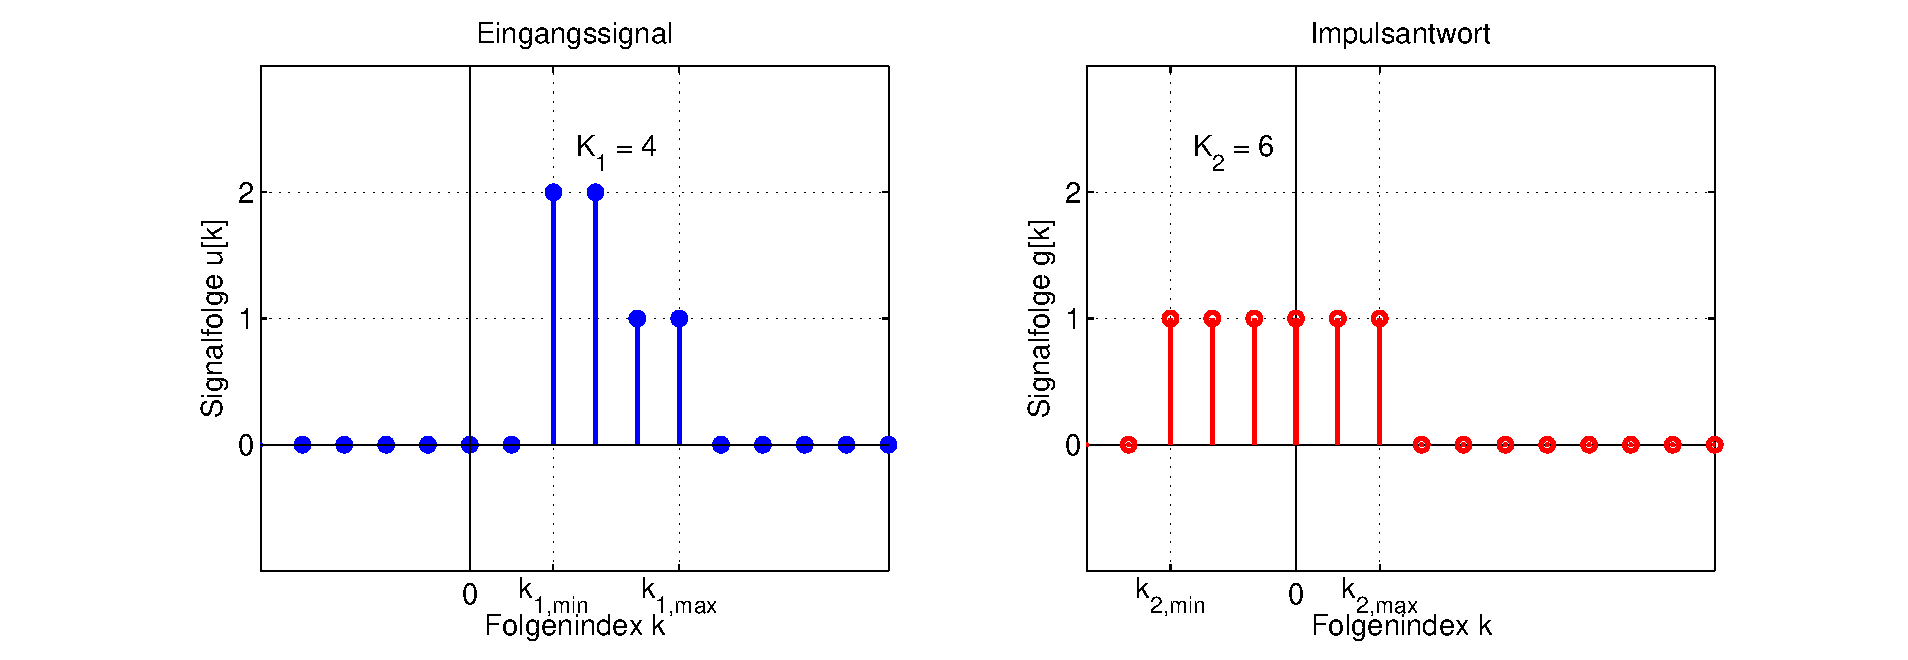
\includegraphics[width=1\textwidth]{Kapitel4/Bilder/image17.eps}}
  \caption{Signalfolgen u[k] und g[k] als Beispiel f\"{u}r die Faltung mit MATLAB}
  \label{fig:FaltungMatlab}
\end{figure}

\noindent Typischerweise werden die Daten nicht mit den f\"{u}hrenden Nullen angegeben, sondern es werden nur die von Null verschiedenen Werte der Signalfolge als Vektor angegeben. So ergeben sich die Vektoren u und g. Die Faltung wird mit dem Befehl conv(u,g) ausgef\"{u}hrt Die Abk\"{u}rzung steht f\"{u}r den englischen Begriff convolution. Der Ergebnisvektor besitzt die L\"{a}nge 

\begin{equation}\label{eq:fouronehundredtwo}
K=K_{1} +K_{2} -1
\end{equation}

\noindent Der Folgenindex startet an der Stelle 

\begin{equation}\label{eq:fouronehundredthree}
k_{MIN} =k_{1,MIN} +k_{2,MIN} 
\end{equation}

\noindent und endet an der Stelle

\begin{equation}\label{eq:fouronehundredfour}
k_{MAX} =k_{MIN} +K_{1} +K_{2} -2
\end{equation}

\noindent In MATLAB kann das Programm wie folgt ausgef\"{u}hrt werden.

\lstinputlisting[caption = {}]{Kapitel4/mat1.m}

\noindent Für das in Bild \ref{fig:FaltungMatlab} dargestellte Beispiel ergibt sich das in Bild \ref{fig:FaltungMatlab1} Ergebnis.

\begin{figure}[H]
  \centerline{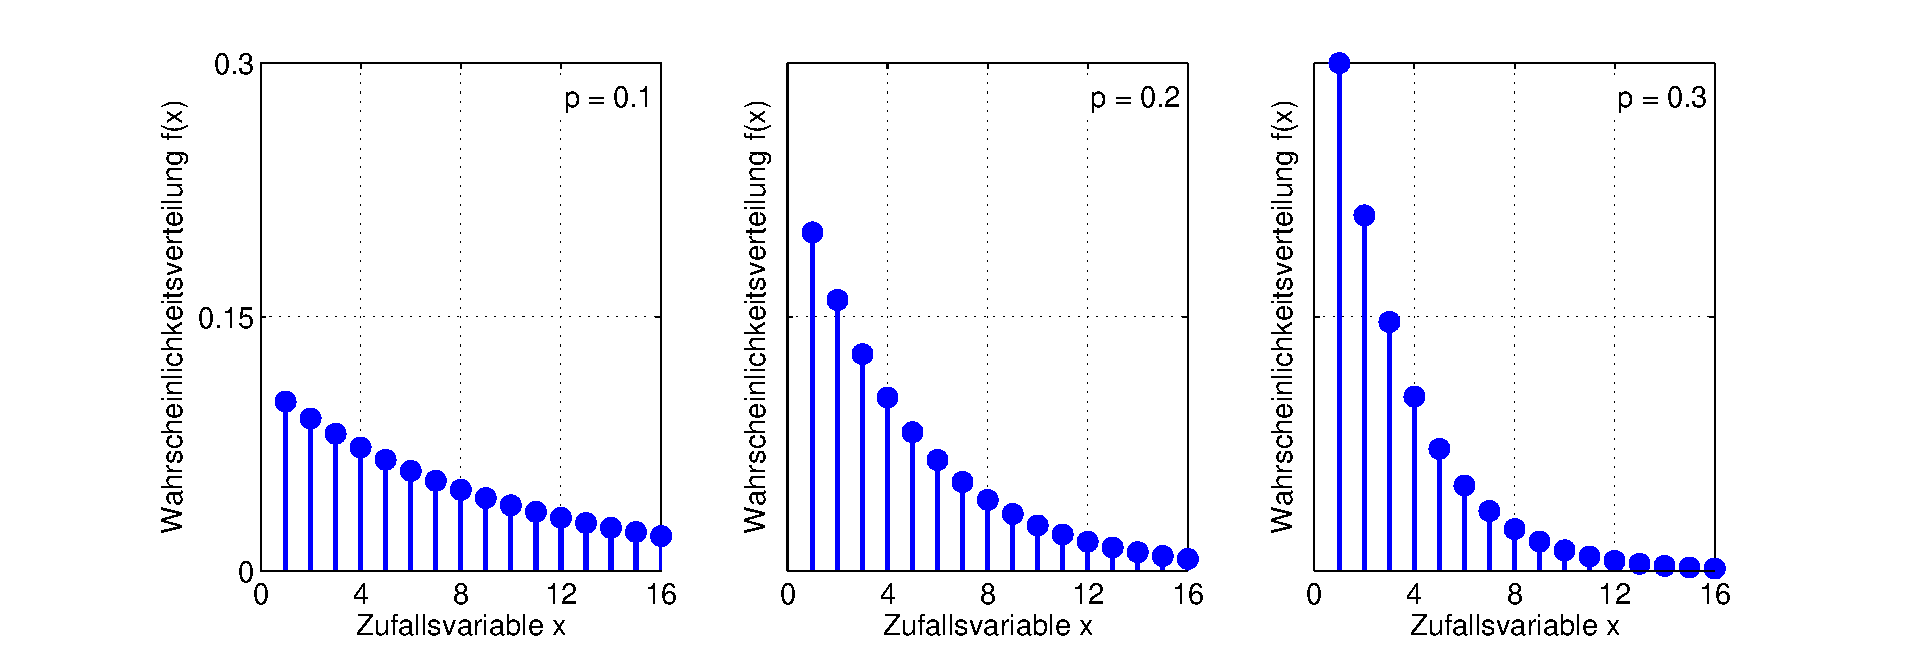
\includegraphics[width=0.5\textwidth]{Kapitel4/Bilder/image18.eps}}
  \caption{Faltung der Signalfolgen u[k] und g[k]}
  \label{fig:FaltungMatlab1}
\end{figure}

\noindent Alle Punkte, die nicht in das Diagramm eingezeichnet sind, sind null.

\clearpage

\subsection{Literatur}

\subsubsection{Literaturstellen mit besonders anschaulicher Darstellung}

\begin{tabular}{|p{0.6in}|p{5.7in}|} \hline 
[Lyon04] & Lyons, Richard G.: Understanding Digital Signal\newline Processing,Prentice Hall, New Jersey, 2004 \\ \hline 
[Stea99] & Stearns, Samuel: Digitale Verarbeitung analoger Signale,\newline 7. Auflage, Oldenbourg Verlag M\"{u}nchen, 1999 \\ \hline 
\end{tabular}


\subsubsection{Literaturstellen mit praktischen Anwendungen}

\begin{tabular}{|p{0.6in}|p{5.7in}|} \hline 
[Wern08] & Werner, Martin: Signale und Systeme,\newline Vieweg Studium Technik, Wiesbaden, 2008 \\ \hline 
[Meye08] & Meyer, Martin: Signalverarbeitung -- Analoge und digitale Signal, Systeme und Filter,\newline Vieweg Studium Technik, Wiesbaden, 2008 \\ \hline 
\end{tabular}


\subsubsection{Literatur zu MATLAB}

\begin{tabular}{|p{0.6in}|p{5.7in}|} \hline 
[Schw07] & Schweizer, Wolfgang: MATLAB kompakt,\newline Oldenbourg Verlag M\"{u}nchen, 2007 \\ \hline 
[Stei07] & Stein, Ulrich: Einstieg in das Programmieren mit MATLAB,\newline Fachbuchverlag Leipzig, 2007 \\ \hline 
\end{tabular}


\subsubsection{Weiterf\"{u}hrende Literatur}

\begin{tabular}{|p{0.6in}|p{5.7in}|} \hline 
[Oppe04] & Oppenheim, Alan: Zeitdiskrete Signalverarbeitung,\newline 2. \"{u}berarbeitete Auflage, Pearson Studium, 2004 \\ \hline 
[Kamm98] & Kammeyer, Karl: Digitale Signalverarbeitung,\newline B.G. Teubner Stuttgart, 1998 \\ \hline 
\end{tabular}